\documentclass[11pt]{article}
% =======================================================================
%   Shared style for CS 300 notes.
%   Usage: place `% =======================================================================
%   Shared style for CS 300 notes.
%   Usage: place `% =======================================================================
%   Shared style for CS 300 notes.
%   Usage: place `\input{../../notes-style.tex}` right after \documentclass
%   in each chapter's lectures.tex and notes.tex.
% =======================================================================

% ---- Layout -----------------------------------------------------------
\usepackage[margin=1in]{geometry}
\usepackage{parskip}        % space between paragraphs, no indent
\usepackage{microtype}      % subtle kerning/spacing improvements

% ---- Colors (muted palette, easy on light-sensitive eyes) -------------
\usepackage{xcolor}
\definecolor{pagebg}       {HTML}{FAF6F0}  % warm cream background
\definecolor{bodyfg}       {HTML}{3D3A36}  % warm dark gray body text
\definecolor{heading}      {HTML}{3D6A6B}  % muted teal
\definecolor{subheading}   {HTML}{5B7A9C}  % dusty blue
\definecolor{accent}       {HTML}{8A6B4A}  % warm tan
\definecolor{linkcol}      {HTML}{5B7A9C}  % same as subheading
\definecolor{mutedtext}    {HTML}{6B6560}  % secondary / caption text
\definecolor{rulecol}      {HTML}{C8BFB0}  % separator / rule

% Callout box palette
\definecolor{defnFrame}    {HTML}{9DB89B}  \definecolor{defnBack}    {HTML}{EEF2E8}
\definecolor{ideaFrame}    {HTML}{9FB4CD}  \definecolor{ideaBack}    {HTML}{E8EEF5}
\definecolor{warnFrame}    {HTML}{CFAE87}  \definecolor{warnBack}    {HTML}{F5EDDF}
\definecolor{noteFrame}    {HTML}{BFA6AE}  \definecolor{noteBack}    {HTML}{F2E8EE}
\definecolor{exFrame}      {HTML}{9FBDBD}  \definecolor{exBack}      {HTML}{E8F0F0}
\definecolor{codeBack}     {HTML}{F3EDE2}
\definecolor{codeBorder}   {HTML}{D4CBBA}
\definecolor{codeKeyword}  {HTML}{6B4F7A}
\definecolor{codeString}   {HTML}{8A6B4A}
\definecolor{codeComment}  {HTML}{8A857F}

% ---- Page background + base text color --------------------------------
\usepackage{pagecolor}
\pagecolor{pagebg}
\color{bodyfg}

% ---- Fonts ------------------------------------------------------------
\usepackage[T1]{fontenc}
\IfFileExists{libertine.sty}{%
    \usepackage{libertine}      % warm, readable serif
    \usepackage[scaled=0.95]{inconsolata}  % softer monospace
}{}

% ---- Hyperref ---------------------------------------------------------
\usepackage{hyperref}
\hypersetup{
    colorlinks=true,
    linkcolor=linkcol,
    urlcolor=linkcol,
    citecolor=linkcol,
    pdfborder={0 0 0},
}

% ---- Section styling --------------------------------------------------
\usepackage[explicit]{titlesec}
\titleformat{\section}
    {\color{heading}\Large\bfseries}
    {\color{heading}\thesection\hspace{0.6em}}{0pt}{#1}
\titleformat{\subsection}
    {\color{subheading}\large\bfseries}
    {\color{subheading}\thesubsection\hspace{0.5em}}{0pt}{#1}
\titleformat{\subsubsection}
    {\color{accent}\normalsize\bfseries}
    {\color{accent}\thesubsubsection\hspace{0.5em}}{0pt}{#1}
\titleformat{\paragraph}[runin]
    {\color{accent}\bfseries}{}{0pt}{#1.}

\titlespacing*{\section}{0pt}{1.6em}{0.6em}
\titlespacing*{\subsection}{0pt}{1.2em}{0.4em}

% ---- Enumerate / itemize spacing --------------------------------------
\usepackage{enumitem}
\setlist[itemize]{leftmargin=1.4em, itemsep=2pt, topsep=4pt}
\setlist[enumerate]{leftmargin=1.6em, itemsep=2pt, topsep=4pt}

% ---- Code listings ----------------------------------------------------
\usepackage{listings}
\lstdefinestyle{notescode}{
    backgroundcolor=\color{codeBack},
    basicstyle=\ttfamily\small\color{bodyfg},
    keywordstyle=\color{codeKeyword}\bfseries,
    stringstyle=\color{codeString},
    commentstyle=\color{codeComment}\itshape,
    frame=single,
    framesep=6pt,
    rulecolor=\color{codeBorder},
    showstringspaces=false,
    breaklines=true,
    xleftmargin=10pt,
    xrightmargin=10pt,
    aboveskip=8pt,
    belowskip=8pt,
}
\lstset{style=notescode}

% ---- Callout boxes (tcolorbox) ----------------------------------------
\usepackage[most]{tcolorbox}

\newtcolorbox{defnbox}[1][]{
    enhanced, breakable,
    colback=defnBack, colframe=defnFrame, coltitle=bodyfg,
    title={\bfseries Definition \textemdash\ #1},
    fonttitle=\bfseries,
    boxrule=0.5pt, arc=2pt, left=8pt, right=8pt, top=6pt, bottom=6pt,
    attach boxed title to top left={xshift=10pt, yshift=-6pt},
    boxed title style={colback=defnFrame, colframe=defnFrame, arc=2pt},
    before skip=8pt, after skip=8pt,
}
\newtcolorbox{ideabox}[1][]{
    enhanced, breakable,
    colback=ideaBack, colframe=ideaFrame, coltitle=bodyfg,
    title={\bfseries Key idea #1},
    boxrule=0.5pt, arc=2pt, left=8pt, right=8pt, top=6pt, bottom=6pt,
    attach boxed title to top left={xshift=10pt, yshift=-6pt},
    boxed title style={colback=ideaFrame, colframe=ideaFrame, arc=2pt},
    before skip=8pt, after skip=8pt,
}
\newtcolorbox{warnbox}[1][]{
    enhanced, breakable,
    colback=warnBack, colframe=warnFrame, coltitle=bodyfg,
    title={\bfseries Gotcha #1},
    boxrule=0.5pt, arc=2pt, left=8pt, right=8pt, top=6pt, bottom=6pt,
    attach boxed title to top left={xshift=10pt, yshift=-6pt},
    boxed title style={colback=warnFrame, colframe=warnFrame, arc=2pt},
    before skip=8pt, after skip=8pt,
}
\newtcolorbox{notebox}[1][]{
    enhanced, breakable,
    colback=noteBack, colframe=noteFrame, coltitle=bodyfg,
    title={\bfseries Aside #1},
    boxrule=0.5pt, arc=2pt, left=8pt, right=8pt, top=6pt, bottom=6pt,
    attach boxed title to top left={xshift=10pt, yshift=-6pt},
    boxed title style={colback=noteFrame, colframe=noteFrame, arc=2pt},
    before skip=8pt, after skip=8pt,
}
\newtcolorbox{examplebox}[1][]{
    enhanced, breakable,
    colback=exBack, colframe=exFrame, coltitle=bodyfg,
    title={\bfseries Example #1},
    boxrule=0.5pt, arc=2pt, left=8pt, right=8pt, top=6pt, bottom=6pt,
    attach boxed title to top left={xshift=10pt, yshift=-6pt},
    boxed title style={colback=exFrame, colframe=exFrame, arc=2pt},
    before skip=8pt, after skip=8pt,
}

% ---- TikZ graph styles (added 2026-04-25 for ch_10 augmentation) ------
% tcolorbox[most] already loads tikz; this block declares the libraries
% + shared `vertex` / `edge` styles used by ch_10's general directed-graph
% diagrams. ch_9's tree-style TikZ uses inline overrides and is
% unaffected. Simple circle nodes + arrow edges only -- no production
% styling.
\usetikzlibrary{arrows.meta, positioning, calc}
\tikzset{
    vertex/.style={circle, draw, minimum size=7mm, inner sep=0pt,
                   font=\small, thick},
    vsource/.style={vertex, fill=ideaBack},
    vdone/.style={vertex, fill=defnBack},
    edge/.style={->, >=Stealth, thick},
    uedge/.style={-, thick},
    treeedge/.style={->, >=Stealth, thick},
    backedge/.style={->, >=Stealth, thick, dashed, red!70!black},
    fwdedge/.style={->, >=Stealth, thick, blue!60!black},
    crossedge/.style={->, >=Stealth, thick, green!50!black, dotted},
    mstedge/.style={-, very thick, accent},
}

% ---- Title block ------------------------------------------------------
\usepackage{titling}
\pretitle{\begin{center}\color{heading}\LARGE\bfseries}
\posttitle{\end{center}\vskip -0.4em}
\preauthor{\begin{center}\color{mutedtext}\normalsize}
\postauthor{\end{center}}
\predate{\begin{center}\color{mutedtext}\small}
\postdate{\end{center}\vspace{0.4em}{\color{rulecol}\hrule height 0.4pt}\vspace{1.2em}}
` right after \documentclass
%   in each chapter's lectures.tex and notes.tex.
% =======================================================================

% ---- Layout -----------------------------------------------------------
\usepackage[margin=1in]{geometry}
\usepackage{parskip}        % space between paragraphs, no indent
\usepackage{microtype}      % subtle kerning/spacing improvements

% ---- Colors (muted palette, easy on light-sensitive eyes) -------------
\usepackage{xcolor}
\definecolor{pagebg}       {HTML}{FAF6F0}  % warm cream background
\definecolor{bodyfg}       {HTML}{3D3A36}  % warm dark gray body text
\definecolor{heading}      {HTML}{3D6A6B}  % muted teal
\definecolor{subheading}   {HTML}{5B7A9C}  % dusty blue
\definecolor{accent}       {HTML}{8A6B4A}  % warm tan
\definecolor{linkcol}      {HTML}{5B7A9C}  % same as subheading
\definecolor{mutedtext}    {HTML}{6B6560}  % secondary / caption text
\definecolor{rulecol}      {HTML}{C8BFB0}  % separator / rule

% Callout box palette
\definecolor{defnFrame}    {HTML}{9DB89B}  \definecolor{defnBack}    {HTML}{EEF2E8}
\definecolor{ideaFrame}    {HTML}{9FB4CD}  \definecolor{ideaBack}    {HTML}{E8EEF5}
\definecolor{warnFrame}    {HTML}{CFAE87}  \definecolor{warnBack}    {HTML}{F5EDDF}
\definecolor{noteFrame}    {HTML}{BFA6AE}  \definecolor{noteBack}    {HTML}{F2E8EE}
\definecolor{exFrame}      {HTML}{9FBDBD}  \definecolor{exBack}      {HTML}{E8F0F0}
\definecolor{codeBack}     {HTML}{F3EDE2}
\definecolor{codeBorder}   {HTML}{D4CBBA}
\definecolor{codeKeyword}  {HTML}{6B4F7A}
\definecolor{codeString}   {HTML}{8A6B4A}
\definecolor{codeComment}  {HTML}{8A857F}

% ---- Page background + base text color --------------------------------
\usepackage{pagecolor}
\pagecolor{pagebg}
\color{bodyfg}

% ---- Fonts ------------------------------------------------------------
\usepackage[T1]{fontenc}
\IfFileExists{libertine.sty}{%
    \usepackage{libertine}      % warm, readable serif
    \usepackage[scaled=0.95]{inconsolata}  % softer monospace
}{}

% ---- Hyperref ---------------------------------------------------------
\usepackage{hyperref}
\hypersetup{
    colorlinks=true,
    linkcolor=linkcol,
    urlcolor=linkcol,
    citecolor=linkcol,
    pdfborder={0 0 0},
}

% ---- Section styling --------------------------------------------------
\usepackage[explicit]{titlesec}
\titleformat{\section}
    {\color{heading}\Large\bfseries}
    {\color{heading}\thesection\hspace{0.6em}}{0pt}{#1}
\titleformat{\subsection}
    {\color{subheading}\large\bfseries}
    {\color{subheading}\thesubsection\hspace{0.5em}}{0pt}{#1}
\titleformat{\subsubsection}
    {\color{accent}\normalsize\bfseries}
    {\color{accent}\thesubsubsection\hspace{0.5em}}{0pt}{#1}
\titleformat{\paragraph}[runin]
    {\color{accent}\bfseries}{}{0pt}{#1.}

\titlespacing*{\section}{0pt}{1.6em}{0.6em}
\titlespacing*{\subsection}{0pt}{1.2em}{0.4em}

% ---- Enumerate / itemize spacing --------------------------------------
\usepackage{enumitem}
\setlist[itemize]{leftmargin=1.4em, itemsep=2pt, topsep=4pt}
\setlist[enumerate]{leftmargin=1.6em, itemsep=2pt, topsep=4pt}

% ---- Code listings ----------------------------------------------------
\usepackage{listings}
\lstdefinestyle{notescode}{
    backgroundcolor=\color{codeBack},
    basicstyle=\ttfamily\small\color{bodyfg},
    keywordstyle=\color{codeKeyword}\bfseries,
    stringstyle=\color{codeString},
    commentstyle=\color{codeComment}\itshape,
    frame=single,
    framesep=6pt,
    rulecolor=\color{codeBorder},
    showstringspaces=false,
    breaklines=true,
    xleftmargin=10pt,
    xrightmargin=10pt,
    aboveskip=8pt,
    belowskip=8pt,
}
\lstset{style=notescode}

% ---- Callout boxes (tcolorbox) ----------------------------------------
\usepackage[most]{tcolorbox}

\newtcolorbox{defnbox}[1][]{
    enhanced, breakable,
    colback=defnBack, colframe=defnFrame, coltitle=bodyfg,
    title={\bfseries Definition \textemdash\ #1},
    fonttitle=\bfseries,
    boxrule=0.5pt, arc=2pt, left=8pt, right=8pt, top=6pt, bottom=6pt,
    attach boxed title to top left={xshift=10pt, yshift=-6pt},
    boxed title style={colback=defnFrame, colframe=defnFrame, arc=2pt},
    before skip=8pt, after skip=8pt,
}
\newtcolorbox{ideabox}[1][]{
    enhanced, breakable,
    colback=ideaBack, colframe=ideaFrame, coltitle=bodyfg,
    title={\bfseries Key idea #1},
    boxrule=0.5pt, arc=2pt, left=8pt, right=8pt, top=6pt, bottom=6pt,
    attach boxed title to top left={xshift=10pt, yshift=-6pt},
    boxed title style={colback=ideaFrame, colframe=ideaFrame, arc=2pt},
    before skip=8pt, after skip=8pt,
}
\newtcolorbox{warnbox}[1][]{
    enhanced, breakable,
    colback=warnBack, colframe=warnFrame, coltitle=bodyfg,
    title={\bfseries Gotcha #1},
    boxrule=0.5pt, arc=2pt, left=8pt, right=8pt, top=6pt, bottom=6pt,
    attach boxed title to top left={xshift=10pt, yshift=-6pt},
    boxed title style={colback=warnFrame, colframe=warnFrame, arc=2pt},
    before skip=8pt, after skip=8pt,
}
\newtcolorbox{notebox}[1][]{
    enhanced, breakable,
    colback=noteBack, colframe=noteFrame, coltitle=bodyfg,
    title={\bfseries Aside #1},
    boxrule=0.5pt, arc=2pt, left=8pt, right=8pt, top=6pt, bottom=6pt,
    attach boxed title to top left={xshift=10pt, yshift=-6pt},
    boxed title style={colback=noteFrame, colframe=noteFrame, arc=2pt},
    before skip=8pt, after skip=8pt,
}
\newtcolorbox{examplebox}[1][]{
    enhanced, breakable,
    colback=exBack, colframe=exFrame, coltitle=bodyfg,
    title={\bfseries Example #1},
    boxrule=0.5pt, arc=2pt, left=8pt, right=8pt, top=6pt, bottom=6pt,
    attach boxed title to top left={xshift=10pt, yshift=-6pt},
    boxed title style={colback=exFrame, colframe=exFrame, arc=2pt},
    before skip=8pt, after skip=8pt,
}

% ---- TikZ graph styles (added 2026-04-25 for ch_10 augmentation) ------
% tcolorbox[most] already loads tikz; this block declares the libraries
% + shared `vertex` / `edge` styles used by ch_10's general directed-graph
% diagrams. ch_9's tree-style TikZ uses inline overrides and is
% unaffected. Simple circle nodes + arrow edges only -- no production
% styling.
\usetikzlibrary{arrows.meta, positioning, calc}
\tikzset{
    vertex/.style={circle, draw, minimum size=7mm, inner sep=0pt,
                   font=\small, thick},
    vsource/.style={vertex, fill=ideaBack},
    vdone/.style={vertex, fill=defnBack},
    edge/.style={->, >=Stealth, thick},
    uedge/.style={-, thick},
    treeedge/.style={->, >=Stealth, thick},
    backedge/.style={->, >=Stealth, thick, dashed, red!70!black},
    fwdedge/.style={->, >=Stealth, thick, blue!60!black},
    crossedge/.style={->, >=Stealth, thick, green!50!black, dotted},
    mstedge/.style={-, very thick, accent},
}

% ---- Title block ------------------------------------------------------
\usepackage{titling}
\pretitle{\begin{center}\color{heading}\LARGE\bfseries}
\posttitle{\end{center}\vskip -0.4em}
\preauthor{\begin{center}\color{mutedtext}\normalsize}
\postauthor{\end{center}}
\predate{\begin{center}\color{mutedtext}\small}
\postdate{\end{center}\vspace{0.4em}{\color{rulecol}\hrule height 0.4pt}\vspace{1.2em}}
` right after \documentclass
%   in each chapter's lectures.tex and notes.tex.
% =======================================================================

% ---- Layout -----------------------------------------------------------
\usepackage[margin=1in]{geometry}
\usepackage{parskip}        % space between paragraphs, no indent
\usepackage{microtype}      % subtle kerning/spacing improvements

% ---- Colors (muted palette, easy on light-sensitive eyes) -------------
\usepackage{xcolor}
\definecolor{pagebg}       {HTML}{FAF6F0}  % warm cream background
\definecolor{bodyfg}       {HTML}{3D3A36}  % warm dark gray body text
\definecolor{heading}      {HTML}{3D6A6B}  % muted teal
\definecolor{subheading}   {HTML}{5B7A9C}  % dusty blue
\definecolor{accent}       {HTML}{8A6B4A}  % warm tan
\definecolor{linkcol}      {HTML}{5B7A9C}  % same as subheading
\definecolor{mutedtext}    {HTML}{6B6560}  % secondary / caption text
\definecolor{rulecol}      {HTML}{C8BFB0}  % separator / rule

% Callout box palette
\definecolor{defnFrame}    {HTML}{9DB89B}  \definecolor{defnBack}    {HTML}{EEF2E8}
\definecolor{ideaFrame}    {HTML}{9FB4CD}  \definecolor{ideaBack}    {HTML}{E8EEF5}
\definecolor{warnFrame}    {HTML}{CFAE87}  \definecolor{warnBack}    {HTML}{F5EDDF}
\definecolor{noteFrame}    {HTML}{BFA6AE}  \definecolor{noteBack}    {HTML}{F2E8EE}
\definecolor{exFrame}      {HTML}{9FBDBD}  \definecolor{exBack}      {HTML}{E8F0F0}
\definecolor{codeBack}     {HTML}{F3EDE2}
\definecolor{codeBorder}   {HTML}{D4CBBA}
\definecolor{codeKeyword}  {HTML}{6B4F7A}
\definecolor{codeString}   {HTML}{8A6B4A}
\definecolor{codeComment}  {HTML}{8A857F}

% ---- Page background + base text color --------------------------------
\usepackage{pagecolor}
\pagecolor{pagebg}
\color{bodyfg}

% ---- Fonts ------------------------------------------------------------
\usepackage[T1]{fontenc}
\IfFileExists{libertine.sty}{%
    \usepackage{libertine}      % warm, readable serif
    \usepackage[scaled=0.95]{inconsolata}  % softer monospace
}{}

% ---- Hyperref ---------------------------------------------------------
\usepackage{hyperref}
\hypersetup{
    colorlinks=true,
    linkcolor=linkcol,
    urlcolor=linkcol,
    citecolor=linkcol,
    pdfborder={0 0 0},
}

% ---- Section styling --------------------------------------------------
\usepackage[explicit]{titlesec}
\titleformat{\section}
    {\color{heading}\Large\bfseries}
    {\color{heading}\thesection\hspace{0.6em}}{0pt}{#1}
\titleformat{\subsection}
    {\color{subheading}\large\bfseries}
    {\color{subheading}\thesubsection\hspace{0.5em}}{0pt}{#1}
\titleformat{\subsubsection}
    {\color{accent}\normalsize\bfseries}
    {\color{accent}\thesubsubsection\hspace{0.5em}}{0pt}{#1}
\titleformat{\paragraph}[runin]
    {\color{accent}\bfseries}{}{0pt}{#1.}

\titlespacing*{\section}{0pt}{1.6em}{0.6em}
\titlespacing*{\subsection}{0pt}{1.2em}{0.4em}

% ---- Enumerate / itemize spacing --------------------------------------
\usepackage{enumitem}
\setlist[itemize]{leftmargin=1.4em, itemsep=2pt, topsep=4pt}
\setlist[enumerate]{leftmargin=1.6em, itemsep=2pt, topsep=4pt}

% ---- Code listings ----------------------------------------------------
\usepackage{listings}
\lstdefinestyle{notescode}{
    backgroundcolor=\color{codeBack},
    basicstyle=\ttfamily\small\color{bodyfg},
    keywordstyle=\color{codeKeyword}\bfseries,
    stringstyle=\color{codeString},
    commentstyle=\color{codeComment}\itshape,
    frame=single,
    framesep=6pt,
    rulecolor=\color{codeBorder},
    showstringspaces=false,
    breaklines=true,
    xleftmargin=10pt,
    xrightmargin=10pt,
    aboveskip=8pt,
    belowskip=8pt,
}
\lstset{style=notescode}

% ---- Callout boxes (tcolorbox) ----------------------------------------
\usepackage[most]{tcolorbox}

\newtcolorbox{defnbox}[1][]{
    enhanced, breakable,
    colback=defnBack, colframe=defnFrame, coltitle=bodyfg,
    title={\bfseries Definition \textemdash\ #1},
    fonttitle=\bfseries,
    boxrule=0.5pt, arc=2pt, left=8pt, right=8pt, top=6pt, bottom=6pt,
    attach boxed title to top left={xshift=10pt, yshift=-6pt},
    boxed title style={colback=defnFrame, colframe=defnFrame, arc=2pt},
    before skip=8pt, after skip=8pt,
}
\newtcolorbox{ideabox}[1][]{
    enhanced, breakable,
    colback=ideaBack, colframe=ideaFrame, coltitle=bodyfg,
    title={\bfseries Key idea #1},
    boxrule=0.5pt, arc=2pt, left=8pt, right=8pt, top=6pt, bottom=6pt,
    attach boxed title to top left={xshift=10pt, yshift=-6pt},
    boxed title style={colback=ideaFrame, colframe=ideaFrame, arc=2pt},
    before skip=8pt, after skip=8pt,
}
\newtcolorbox{warnbox}[1][]{
    enhanced, breakable,
    colback=warnBack, colframe=warnFrame, coltitle=bodyfg,
    title={\bfseries Gotcha #1},
    boxrule=0.5pt, arc=2pt, left=8pt, right=8pt, top=6pt, bottom=6pt,
    attach boxed title to top left={xshift=10pt, yshift=-6pt},
    boxed title style={colback=warnFrame, colframe=warnFrame, arc=2pt},
    before skip=8pt, after skip=8pt,
}
\newtcolorbox{notebox}[1][]{
    enhanced, breakable,
    colback=noteBack, colframe=noteFrame, coltitle=bodyfg,
    title={\bfseries Aside #1},
    boxrule=0.5pt, arc=2pt, left=8pt, right=8pt, top=6pt, bottom=6pt,
    attach boxed title to top left={xshift=10pt, yshift=-6pt},
    boxed title style={colback=noteFrame, colframe=noteFrame, arc=2pt},
    before skip=8pt, after skip=8pt,
}
\newtcolorbox{examplebox}[1][]{
    enhanced, breakable,
    colback=exBack, colframe=exFrame, coltitle=bodyfg,
    title={\bfseries Example #1},
    boxrule=0.5pt, arc=2pt, left=8pt, right=8pt, top=6pt, bottom=6pt,
    attach boxed title to top left={xshift=10pt, yshift=-6pt},
    boxed title style={colback=exFrame, colframe=exFrame, arc=2pt},
    before skip=8pt, after skip=8pt,
}

% ---- TikZ graph styles (added 2026-04-25 for ch_10 augmentation) ------
% tcolorbox[most] already loads tikz; this block declares the libraries
% + shared `vertex` / `edge` styles used by ch_10's general directed-graph
% diagrams. ch_9's tree-style TikZ uses inline overrides and is
% unaffected. Simple circle nodes + arrow edges only -- no production
% styling.
\usetikzlibrary{arrows.meta, positioning, calc}
\tikzset{
    vertex/.style={circle, draw, minimum size=7mm, inner sep=0pt,
                   font=\small, thick},
    vsource/.style={vertex, fill=ideaBack},
    vdone/.style={vertex, fill=defnBack},
    edge/.style={->, >=Stealth, thick},
    uedge/.style={-, thick},
    treeedge/.style={->, >=Stealth, thick},
    backedge/.style={->, >=Stealth, thick, dashed, red!70!black},
    fwdedge/.style={->, >=Stealth, thick, blue!60!black},
    crossedge/.style={->, >=Stealth, thick, green!50!black, dotted},
    mstedge/.style={-, very thick, accent},
}

% ---- Title block ------------------------------------------------------
\usepackage{titling}
\pretitle{\begin{center}\color{heading}\LARGE\bfseries}
\posttitle{\end{center}\vskip -0.4em}
\preauthor{\begin{center}\color{mutedtext}\normalsize}
\postauthor{\end{center}}
\predate{\begin{center}\color{mutedtext}\small}
\postdate{\end{center}\vspace{0.4em}{\color{rulecol}\hrule height 0.4pt}\vspace{1.2em}}


\title{CS 300 -- Chapter 10 Lectures\\\large Graphs}
\author{Jose de Lima}
\date{\today}

\begin{document}
\maketitle

\begin{ideabox}[Chapter map]
\textbf{Where this sits in CS 300.} Chapter 10 is the
\emph{abstraction-substrate chapter}. Every previous data structure in
this course is really a specialization of a graph: a linked list is a
path, a tree is a connected acyclic graph, a heap is a tree with an
ordering, a hash-chained bucket is a forest. Chapter 10 turns that
specialization upside down --- we work directly with the most general
model of ``structured connections'' and learn the algorithms that live
on it: shortest paths, scheduling, dependency resolution, MST,
all-pairs distances, strongly connected components. Builds on
\textbf{ch.~6} (BSTs are connected acyclic graphs), \textbf{ch.~7}
(the priority queue is the substrate Dijkstra rides on), and
\textbf{ch.~9} (parent-pointer trees are exactly what BFS and DFS
emit).

\textbf{What you add to your toolkit:}
\begin{itemize}
    \item \textbf{Two graph representations} and when to pick which:
          adjacency list for sparse graphs ($O(V+E)$ space,
          $O(\deg u)$ neighbour scan), adjacency matrix for dense or
          all-pairs work ($O(V^2)$ space, $O(1)$ edge query). The
          \emph{first} question to ask about any graph algorithm is
          ``what does this cost on a sparse input?''
    \item \textbf{BFS as ``shortest paths in unweighted graphs''}
          plus the layer-monotonicity argument that proves it.
          BFS is the unique algorithm whose frontier ordering equals
          its correctness proof.
    \item \textbf{DFS plus edge classification} (tree / back / forward
          / cross). One simple DFS run, four downstream algorithms:
          cycle detection (back edge $\Rightarrow$ cycle),
          topological sort (post-order reversal), strongly connected
          components (Kosaraju's two-pass), articulation points
          (tree-edge / back-edge interplay).
    \item \textbf{Relaxation as the universal SSSP primitive.}
          Dijkstra, Bellman-Ford, and DAG-relax are all instances of
          ``relax every edge in some order; correctness comes from
          the order.'' Internalise the primitive and the three
          algorithms collapse to one.
    \item \textbf{Cut and cycle properties} as the structural lemmas
          that justify both Kruskal and Prim --- the same proof
          carrying two different greedy implementations.
    \item \textbf{Algorithm selection at a glance:} given a problem
          (single-pair / single-source / all-pairs / MST / topo /
          cycle / SCC) and graph properties (unweighted /
          non-negative / negative-no-cycle / negative-with-cycle /
          DAG / sparse / dense), pick the right algorithm in one
          sentence. Master decision table is \S10.15.
\end{itemize}

\textbf{Mastery checklist} --- you should be able to, without
references:
\begin{enumerate}
    \item State the BFS algorithm + sketch why it produces shortest
          paths in unweighted graphs (\S10.5 layer-monotonicity
          argument: queue contents are
          $\{d, \ldots, d, d+1, \ldots\}$ stretches, alternative
          paths would have surfaced earlier and shorter).
    \item Run DFS on a 6-node directed graph by hand, classifying
          every edge as tree / back / forward / cross + identifying
          the topological sort from post-order
          (\S10.6 + \S10.11).
    \item State \textbf{relaxation} + argue why it is monotonic +
          sketch why one round of relaxation over all edges in
          topological order solves DAG shortest paths in $O(V+E)$
          (\S10.8 universal-SSSP-primitive framing).
    \item State Dijkstra's algorithm + why it requires non-negative
          edge weights, with a one-line counterexample on a 3-node
          graph with a negative edge (\S10.9 greedy-correctness
          argument + \S10.9 negative-edge counterexample).
    \item State Bellman-Ford's $|V|-1$-round relaxation correctness
          (induction on path length) + describe negative-cycle
          detection (one extra round; any further relaxation
          $\Rightarrow$ reachable negative cycle), per \S10.10.
    \item State the \textbf{cut property} + \textbf{cycle property}
          + use them to argue both Kruskal and Prim produce a minimum
          spanning tree (\S10.12).
    \item Pick the right algorithm for a shortest-path problem at
          first sight: unweighted $\to$ BFS, DAG $\to$ DAG-relax,
          non-negative-weighted $\to$ Dijkstra, negative weights
          $\to$ Bellman-Ford, all-pairs $\to$ Floyd-Warshall (or
          Johnson for sparse). Justify each choice in one sentence
          (\S10.15 master decision table).
\end{enumerate}

\textbf{Looking ahead.} Chapter 11 introduces \textbf{B-trees} as
the shallow-and-wide alternative to ch.~9's balanced BSTs ---
filesystems and database indices use B-trees because the disk-page /
SSD-block geometry rewards high fan-out, and the underlying
graph-flavoured pointer structure is the same one we manipulate
here. Chapter 12 covers the \textbf{set ADT} in full; the
\texttt{visited} / \texttt{discovered} sets that BFS and DFS rely on
are exactly the ``does the set contain $x$?'' interface ch.~12
formalises. \textbf{Forward direction} (not in cs-300): A* (Dijkstra
+ heuristic, \S10.16 notebox), Johnson's algorithm (sparse all-pairs,
\S10.16), network flow (Ford-Fulkerson + Edmonds-Karp, CLRS Ch~26),
planar graphs (4-colour theorem, planarity testing).
\end{ideabox}

\begin{ideabox}
\textbf{Why graphs matter.} Once your problem is ``these things
connect to those things,'' you're working with a graph. Graphs are
the most general model of ``structured connections,'' so they're
where interesting algorithms live: shortest paths, scheduling,
routing, dependency resolution, network flow, recommendation,
social analysis. You'll use them more than any other data structure
in the wild.
\end{ideabox}

\section{10.1 Introduction}

\subsection*{The vocabulary}

\begin{defnbox}
\textbf{Graph.} A pair $G = (V, E)$ where $V$ is a set of \emph{vertices} (nodes) and $E$ is a set of \emph{edges}, each edge connecting two vertices.

\textbf{Adjacent.} Two vertices are adjacent if an edge connects them.

\textbf{Path.} A sequence of edges from a source vertex to a destination vertex. The \emph{length} of a path is the number of edges (or the sum of edge weights, for weighted graphs).

\textbf{Distance.} The length of the \emph{shortest} path between two vertices.

\textbf{$|V|$ and $|E|$.} The number of vertices and edges. By convention, algorithms are analyzed as a function of both; the abbreviations $V$ and $E$ appear inside Big-O notation.
\end{defnbox}

\begin{notebox}
Watch the word ``length'' -- it's overloaded. An \emph{unweighted} path length is a count of edges; a \emph{weighted} path length is a sum of weights. When someone says ``shortest path'' without qualifying, they usually mean the weighted version unless context makes it obvious.
\end{notebox}

\subsection*{The shape of the space}

A graph has up to $\binom{V}{2} = \Theta(V^2)$ possible edges (undirected) or $V(V-1) = \Theta(V^2)$ (directed). The real world rarely fills that space:

\begin{itemize}[leftmargin=*]
    \item \textbf{Dense graph}: $|E| = \Theta(V^2)$. Every vertex is connected to a constant fraction of the others. Complete graphs, small road networks within a city block.
    \item \textbf{Sparse graph}: $|E| = O(V)$ or $O(V \log V)$. Each vertex has only a few neighbors. Most real graphs: social networks, road networks, computer networks, the web.
\end{itemize}

Dense vs.\ sparse matters \emph{enormously} for algorithm choice. An $O(V^2)$ algorithm on a sparse graph is wasteful; an $O(E \log V)$ algorithm is brilliant on sparse graphs and mediocre on dense ones. The first question to ask about any graph algorithm is: ``what does this cost on a sparse input?''

\begin{examplebox}
\textbf{Concrete numbers.} Facebook has roughly $3 \times 10^9$ users and an average of a few hundred friends per user. That's $V = 3 \times 10^9$, $E \approx 10^{12}$. The dense upper bound would be $V^2 \approx 9 \times 10^{18}$ -- seven orders of magnitude larger. An adjacency matrix is physically impossible; an adjacency list is plausible. This is why sparsity assumptions drive the design of real graph systems.
\end{examplebox}

\subsection*{The picture}

Vocabulary is easier to keep straight if you can see it. The same
five vertices below carry an undirected and a directed edge set;
note how ``degree'' splits into ``in-degree'' and ``out-degree'' once
edges acquire direction.

\begin{center}
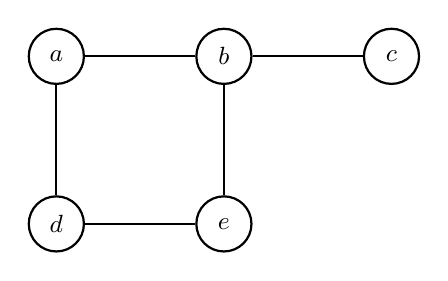
\begin{tikzpicture}[node distance=14mm]
    \node[vertex] (a) {$a$};
    \node[vertex, right=of a] (b) {$b$};
    \node[vertex, right=of b] (c) {$c$};
    \node[vertex, below=of a] (d) {$d$};
    \node[vertex, below=of b] (e) {$e$};
    \draw[uedge] (a) -- (b);
    \draw[uedge] (b) -- (c);
    \draw[uedge] (a) -- (d);
    \draw[uedge] (b) -- (e);
    \draw[uedge] (d) -- (e);
\end{tikzpicture}
\quad
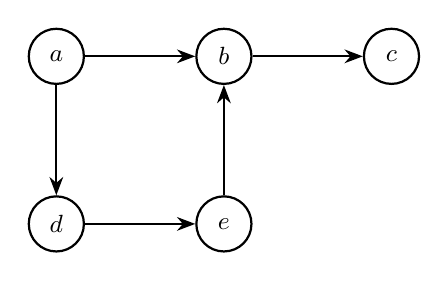
\begin{tikzpicture}[node distance=14mm]
    \node[vertex] (a) {$a$};
    \node[vertex, right=of a] (b) {$b$};
    \node[vertex, right=of b] (c) {$c$};
    \node[vertex, below=of a] (d) {$d$};
    \node[vertex, below=of b] (e) {$e$};
    \draw[edge] (a) -- (b);
    \draw[edge] (b) -- (c);
    \draw[edge] (a) -- (d);
    \draw[edge] (e) -- (b);
    \draw[edge] (d) -- (e);
\end{tikzpicture}
\end{center}

Left (undirected): vertex $b$ has \emph{degree} $3$ ---
neighbours $\{a, c, e\}$. Path $a$--$d$--$e$--$b$ has length $3$
(unweighted).

Right (directed): vertex $b$ has \emph{in-degree} $2$ (edges from
$a$ and $e$) and \emph{out-degree} $1$ (edge to $c$). Vertex $a$
is a \emph{source} (in-degree $0$); vertex $c$ is a \emph{sink}
(out-degree $0$). The directed path $a \to d \to e \to b \to c$
has length $4$.

\section{10.2 Applications}

The textbook section runs through three examples; the interesting claim is the same in each:

\begin{ideabox}
\textbf{Graphs model anything with binary relationships.} Once your problem is ``these things connect to those things,'' you're working with a graph. The graph abstraction is so ubiquitous that recognizing it in a problem is 90\% of the solution.
\end{ideabox}

\subsection*{Navigation (geography)}

Cities/intersections are vertices; roads are edges. Edge weights are distances or travel times. Shortest-path queries give driving directions. This is what powers Google Maps, Waze, and every GPS unit made since the 90s.

The interesting twist: edge weights aren't static. Real-time traffic turns the same road into a different edge every few minutes. The right algorithm has to be fast enough that you can \emph{re-solve} every time conditions change, not just once.

\subsection*{Product recommendations (e-commerce)}

Products are vertices; ``bought together'' or ``viewed together'' is an edge. A customer's basket gives you a starting set; walk one step out along the edges and you have recommendations.

\subsection*{Social and professional networks}

People are vertices; relationships are edges. ``Friends of friends'' is a two-step walk. PageRank, centrality, community detection all live here.

\subsection*{Other common models you'll encounter}

\begin{itemize}[leftmargin=*]
    \item \textbf{Compiler dependencies.} Source files are vertices, \texttt{\#include} edges drive rebuild order -- a topological sort of the dependency DAG.
    \item \textbf{Spreadsheet formula dependencies.} Cells are vertices, references are edges. Evaluation order is a topological sort; circular references are a cycle detection problem.
    \item \textbf{Package managers.} Libraries are vertices, dependency constraints are edges. Resolving versions is a constraint problem on the graph.
    \item \textbf{Build systems (\texttt{make}, \texttt{bazel}, \texttt{cmake}).} Targets are vertices, prerequisites are edges. Determining what to rebuild after a change is reachability.
    \item \textbf{State machines.} States are vertices, transitions are edges. Model checking is graph reachability with labels.
    \item \textbf{Game AI and pathfinding.} Tiles or waypoints are vertices, valid moves are edges. A* (shortest path with a heuristic) is the industry standard.
    \item \textbf{Neural networks.} The topology is literally a weighted DAG.
\end{itemize}

\begin{notebox}
If you can phrase your problem as ``given these things and these connections, what can I reach / what's the best path / what's the order / which connections matter,'' stop trying to invent algorithms and go find the right graph algorithm instead. That's the whole payoff of the abstraction.
\end{notebox}

\section{10.3 Adjacency Lists}

We have the vocabulary. Now: how do we store a graph in memory?

\begin{defnbox}
\textbf{Adjacency list.} Each vertex carries a list (or vector) of the vertices it's adjacent to. One list per vertex.
\end{defnbox}

\subsection*{C++ representations}

Several idioms are common; pick based on your data model.

\begin{lstlisting}[basicstyle=\ttfamily\small,frame=single]
// 1. Vertices as integer IDs 0..V-1, parallel array of neighbor vectors.
//    The fastest and most common choice in competitive programming.
std::vector<std::vector<int>> adj(V);
adj[u].push_back(v);   // add edge u--v
adj[v].push_back(u);   // undirected => add to both lists

// 2. Weighted edges: store (neighbor, weight) pairs.
std::vector<std::vector<std::pair<int,int>>> adj(V);
adj[u].emplace_back(v, weight);

// 3. Vertex objects with owned adjacency data (OOP style).
struct Vertex {
    std::string label;
    std::vector<Vertex*> neighbors;
};
\end{lstlisting}

\subsection*{Cost analysis}

\begin{itemize}[leftmargin=*]
    \item \textbf{Space}: $O(V + E)$. Each vertex's list contributes one header; each edge contributes two list entries (one in each endpoint's list for undirected graphs).
    \item \textbf{``Is $u$ adjacent to $v$?''}: $O(\deg(u))$. Scan $u$'s list. Worst case $O(V)$ if $u$ is connected to everything.
    \item \textbf{``List all neighbors of $u$''}: $O(\deg(u))$. Perfect -- you just hand over the list.
    \item \textbf{Add/remove edge}: $O(1)$ to add. Removal is $O(\deg(u))$ because you have to find the entry.
\end{itemize}

\begin{ideabox}
Adjacency lists are the default choice for sparse graphs. The space win ($V + E$ vs.\ $V^2$) is so large that even the slower adjacency query is usually tolerated. Essentially every production graph library (NetworkX, boost::graph, the JDK's graph APIs) uses lists by default.
\end{ideabox}

\begin{notebox}
\textbf{Adjacency \emph{set} vs.\ adjacency \emph{list}.} MIT 6.006
prefers an adjacency \emph{set}: a Python \texttt{set} per vertex
(or an \texttt{std::unordered\_set<int>} per vertex in C++). The
trade-off is on the ``is $u$ adjacent to $v$?'' query:

\begin{itemize}[leftmargin=*]
    \item Adjacency \emph{list} (vector of neighbours): edge query
          is $O(\deg u)$ scan; iteration is cache-friendly +
          $O(\deg u)$.
    \item Adjacency \emph{set} (hash set of neighbours): edge query
          is $O(1)$ \emph{expected}; iteration is $O(\deg u)$ with
          worse constants (hash-bucket walk).
\end{itemize}

In competitive programming and most production C++ the list form
wins on constants for small/medium $\deg u$ --- BFS, DFS, Dijkstra
all rely on neighbour iteration, not on point edge queries. Reach
for the set form when the algorithm asks ``is $(u,v)$ an edge?''
many times and the graph is too sparse to justify a matrix. The
chapter from here on uses the list form.
\end{notebox}

\section{10.4 Adjacency Matrices}

\begin{defnbox}
\textbf{Adjacency matrix.} A $V \times V$ matrix $M$ where $M[i][j] = 1$ if there's an edge from $i$ to $j$, else $0$. For weighted graphs, $M[i][j]$ holds the weight (with $\infty$ or some sentinel for ``no edge'').
\end{defnbox}

\begin{lstlisting}[basicstyle=\ttfamily\small,frame=single]
std::vector<std::vector<int>> m(V, std::vector<int>(V, 0));
m[u][v] = 1;
m[v][u] = 1;   // undirected

// Weighted version; INT_MAX = "no edge"
std::vector<std::vector<int>> w(V, std::vector<int>(V, INT_MAX));
w[i][i] = 0;   // zero distance to self
w[u][v] = weight;
\end{lstlisting}

\subsection*{Cost analysis}

\begin{itemize}[leftmargin=*]
    \item \textbf{Space}: $\Theta(V^2)$. Forgiving for small dense graphs, catastrophic for large sparse ones.
    \item \textbf{``Is $u$ adjacent to $v$?''}: $O(1)$. Just read the matrix cell.
    \item \textbf{``List all neighbors of $u$''}: $O(V)$. Scan row $u$ even if there are only two neighbors.
    \item \textbf{Add/remove edge}: $O(1)$.
    \item \textbf{Matrix math}: $M^k[i][j]$ is the number of length-$k$ walks from $i$ to $j$. This is the basis of matrix-multiplication shortest-path algorithms and a ton of algebraic graph theory.
\end{itemize}

\subsection*{When to pick which}

\begin{center}
\begin{tabular}{lll}
\hline
& Adjacency list & Adjacency matrix \\
\hline
Space & $O(V+E)$ & $\Theta(V^2)$ \\
Edge query $(u,v)?$ & $O(\deg u)$ & $O(1)$ \\
List neighbors of $u$ & $O(\deg u)$ & $O(V)$ \\
Iterate all edges & $O(V+E)$ & $O(V^2)$ \\
Good for... & sparse, large $V$ & dense, small $V$ \\
\hline
\end{tabular}
\end{center}

\begin{warnbox}
The $V^2$ space blow-up of an adjacency matrix is lethal well before $V$ seems ``large.'' At $V = 10^5$, a matrix of \texttt{int} costs 40 GB; at $V = 10^6$, it's 4 TB. Adjacency lists happily hold the same data in kilobytes or megabytes, depending on edge count. \emph{Always check sparsity before reaching for a matrix.}
\end{warnbox}

\begin{notebox}
A third representation worth knowing is the \textbf{edge list}: just \texttt{std::vector<Edge>} with no per-vertex indexing. Useless for most queries, but perfect for Kruskal's MST algorithm (which processes edges in weight order) and for streaming graphs through a network.
\end{notebox}

\section{10.5 Breadth-First Search}

\begin{ideabox}
\textbf{BFS in one sentence.} Explore vertices in order of distance from the start: all distance-1 vertices before any distance-2, all distance-2 before any distance-3, and so on. The queue \emph{is} the algorithm -- FIFO ordering is what produces the distance-layered traversal.
\end{ideabox}

\subsection*{Algorithm}

\begin{lstlisting}[basicstyle=\ttfamily\small,frame=single]
void bfs(const std::vector<std::vector<int>>& adj, int start) {
    std::vector<bool> discovered(adj.size(), false);
    std::queue<int> frontier;

    frontier.push(start);
    discovered[start] = true;

    while (!frontier.empty()) {
        int u = frontier.front(); frontier.pop();
        visit(u);
        for (int v : adj[u]) {
            if (!discovered[v]) {
                discovered[v] = true;
                frontier.push(v);
            }
        }
    }
}
\end{lstlisting}

\begin{warnbox}
\textbf{Mark on enqueue, not on dequeue.} The \texttt{discovered} flag is set \emph{when a vertex is pushed}, not when it's popped. If you mark on pop, the same vertex can be pushed many times through different neighbors, blowing up the queue. The ``mark on enqueue'' invariant guarantees each vertex is pushed exactly once.
\end{warnbox}

\subsection*{Distance and parent tracking}

BFS's real power isn't just ``visit everything.'' It computes \emph{shortest paths in unweighted graphs} for free. Augment each visited vertex with a distance and a parent pointer:

\begin{lstlisting}[basicstyle=\ttfamily\small,frame=single]
void bfs(const std::vector<std::vector<int>>& adj, int start,
         std::vector<int>& dist, std::vector<int>& parent) {
    int n = adj.size();
    dist.assign(n, -1);
    parent.assign(n, -1);
    std::queue<int> q;
    q.push(start);
    dist[start] = 0;
    while (!q.empty()) {
        int u = q.front(); q.pop();
        for (int v : adj[u]) {
            if (dist[v] == -1) {
                dist[v] = dist[u] + 1;
                parent[v] = u;
                q.push(v);
            }
        }
    }
}
\end{lstlisting}

After BFS, \texttt{dist[v]} is the minimum number of edges from \texttt{start} to \texttt{v}; following \texttt{parent} pointers back from \texttt{v} reconstructs the path in reverse.

\subsection*{Cost}

$O(V + E)$. Each vertex is dequeued once; each edge is scanned at most twice (once from each endpoint, for undirected graphs). Can't be beat for unweighted shortest paths.

\subsection*{Why BFS works -- the invariant}

\begin{ideabox}
At any point in BFS, the queue contains vertices at distances $\{d, d, \ldots, d, d+1, d+1, \ldots\}$ -- a stretch of one layer, then the next. When a layer-$d$ vertex is popped, its yet-undiscovered neighbors are exactly the layer-$d+1$ vertices reachable through it, and they go to the back of the queue. That's why the FIFO ordering preserves ``shortest path''-ness -- any alternative path would have been seen (and shorter) on an earlier iteration.
\end{ideabox}

\begin{notebox}
\textbf{Layer-monotonicity proof.} Define $L_d = \{v : \texttt{dist}[v] = d\}$ as
the set of vertices at distance $d$ from the source. Claim: BFS
discovers vertices in non-decreasing order of distance --- the queue
is at all times a non-decreasing sequence of \texttt{dist} values
spanning at most two consecutive layers.

\emph{Induction on $d$.} \textsc{Base} ($d = 0$): the source is
pushed first, with $\texttt{dist} = 0$, and the queue holds only
$L_0$. \textsc{Step} ($d \to d{+}1$): suppose the invariant holds
when the first $L_d$-vertex is about to be popped, so the queue is
$L_d \mathbin\Vert L_{d+1}^{\text{partial}}$. Popping a $u \in L_d$
and scanning its neighbours either finds an already-discovered
vertex (skip) or an undiscovered $v$. Any neighbour of $u$ has
$\texttt{dist}[v] \le \texttt{dist}[u] + 1 = d + 1$. If
$\texttt{dist}[v] < d+1$ it would already be discovered (the source
would have reached it via a shorter path, processed earlier under
the IH). So $\texttt{dist}[v] = d+1$, $v$ joins the back of the
queue, and the invariant is preserved.

The invariant immediately gives shortest paths: when $v$ is
\emph{first} discovered, the assignment $\texttt{dist}[v] =
\texttt{dist}[u] + 1$ records the smallest possible distance
because any shorter path would have made $v$ visible from a
\emph{shallower} layer, contradicting ``$v$ undiscovered until
now.''
\end{notebox}

\subsection*{Parent pointers and the BFS tree}

The \texttt{parent[]} array isn't just bookkeeping --- it builds a
\textbf{BFS tree} rooted at the source: every reachable vertex $v$
has exactly one parent, namely the vertex from which $v$ was first
discovered. The tree's edges are exactly the ``$v$ first discovered
from $u$'' edges, and the tree's root-to-$v$ path is a shortest
$s \to v$ path in the original graph (length $= \texttt{dist}[v]$).

This is the BFS analogue of ch.~9's parent-pointer trees ---
\emph{the parent pointers \emph{are} the data structure BFS produces.}
Two callers of BFS use it differently:
\begin{itemize}[leftmargin=*]
    \item ``Shortest path'' callers walk parent pointers backward
          from the target (\texttt{path.push\_back(prev[v])} in a
          loop, then \texttt{std::reverse}). $O(\text{path length})$
          per query, no extra preprocessing.
    \item ``Component'' callers ignore the tree and just iterate
          over \texttt{dist[]} for ``everyone reachable from $s$.''
\end{itemize}

\begin{center}
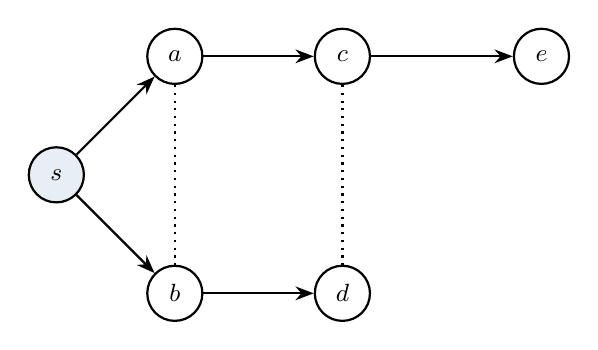
\begin{tikzpicture}[node distance=14mm]
    \node[vsource] (s) {$s$};
    \node[vertex, above right=of s] (a) {$a$};
    \node[vertex, below right=of s] (b) {$b$};
    \node[vertex, right=of a] (c) {$c$};
    \node[vertex, right=of b] (d) {$d$};
    \node[vertex, right=18mm of c] (e) {$e$};
    % BFS-tree edges (solid)
    \draw[treeedge] (s) -- (a);
    \draw[treeedge] (s) -- (b);
    \draw[treeedge] (a) -- (c);
    \draw[treeedge] (b) -- (d);
    \draw[treeedge] (c) -- (e);
    % Non-tree edges (dotted) -- short-circuits the BFS skipped
    \draw[uedge, dotted] (a) -- (b);
    \draw[uedge, dotted] (c) -- (d);
\end{tikzpicture}
\end{center}

\emph{BFS tree on a 6-vertex undirected graph,} source $s$ at the
left. Layer $L_0 = \{s\}$, $L_1 = \{a, b\}$, $L_2 = \{c, d\}$,
$L_3 = \{e\}$. Solid arrows are the parent-pointer edges BFS keeps;
dotted edges $(a, b)$ and $(c, d)$ are present in the input graph
but are \emph{not} added to the BFS tree because their endpoints
were already in the same or adjacent layer when the second endpoint
was first discovered.

\begin{examplebox}
\textbf{BFS trace.} Run BFS from $s$ on the 6-vertex graph above
with adjacency lists $\texttt{adj}[s] = [a, b]$,
$\texttt{adj}[a] = [s, b, c]$, $\texttt{adj}[b] = [s, a, d]$,
$\texttt{adj}[c] = [a, d, e]$, $\texttt{adj}[d] = [b, c]$,
$\texttt{adj}[e] = [c]$.

\medskip
\begin{tabular}{rp{6.5cm}|l|l}
\hline
Step & action & $\texttt{dist}[s,a,b,c,d,e]$ & queue \\
\hline
0 & init & $0,-,-,-,-,-$ & $[s]$ \\
1 & pop $s$, push $a, b$ & $0,1,1,-,-,-$ & $[a, b]$ \\
2 & pop $a$, push $c$ ($b$ already disc.) & $0,1,1,2,-,-$ & $[b, c]$ \\
3 & pop $b$, push $d$ ($a$ already disc.) & $0,1,1,2,2,-$ & $[c, d]$ \\
4 & pop $c$, push $e$ ($a, d$ already disc.) & $0,1,1,2,2,3$ & $[d, e]$ \\
5 & pop $d$ (all neighbours discovered) & $0,1,1,2,2,3$ & $[e]$ \\
6 & pop $e$ (sole neighbour discovered) & $0,1,1,2,2,3$ & $[\,]$ \\
\hline
\end{tabular}

\medskip
Final \texttt{dist} array matches the layer assignment from the
diagram. Parent pointers track which layer-$d$ vertex first reached
each layer-$(d{+}1)$ neighbour. Note step 4: $a$ and $d$ are already
discovered so $c$'s edges to them \emph{don't} extend the BFS tree
--- those become the dotted non-tree edges in the figure.
\end{examplebox}

\subsection*{Typical applications}

\begin{itemize}[leftmargin=*]
    \item \textbf{Shortest path in unweighted graph} -- unbeatable.
    \item \textbf{``Friend of a friend'' recommendations} -- explore distance-2 and distance-3 neighborhoods.
    \item \textbf{Connected components} -- run BFS from every unvisited vertex; each run finds one component.
    \item \textbf{Bipartite check} -- 2-color BFS layers; if an edge connects two same-colored vertices, the graph isn't bipartite.
    \item \textbf{Crawling / scraping} -- explore a website or peer-to-peer network level-by-level.
    \item \textbf{Closest-of-many search} -- as in the peer-to-peer example above, find the first node satisfying a condition (fewest hops).
\end{itemize}

\section{10.6 Depth-First Search}

\begin{ideabox}
\textbf{DFS in one sentence.} Go as far as possible along one path, backtrack only when stuck. A stack (explicit or the call stack) \emph{is} the algorithm.
\end{ideabox}

\subsection*{Iterative DFS}

\begin{lstlisting}[basicstyle=\ttfamily\small,frame=single]
void dfs(const std::vector<std::vector<int>>& adj, int start) {
    std::vector<bool> visited(adj.size(), false);
    std::stack<int> s;
    s.push(start);

    while (!s.empty()) {
        int u = s.top(); s.pop();
        if (visited[u]) continue;
        visited[u] = true;
        visit(u);
        for (int v : adj[u])
            if (!visited[v]) s.push(v);
    }
}
\end{lstlisting}

\begin{warnbox}
\textbf{Iterative DFS marks on pop, not on push.} The opposite of BFS. If you mark on push with a stack, the neighbor ordering gets reversed in a subtle way that most people trip over. The idiomatic iterative form above pushes liberally and filters at the top of the loop; duplicate stack entries are OK.
\end{warnbox}

\subsection*{Recursive DFS}

Shorter and usually what you want:

\begin{lstlisting}[basicstyle=\ttfamily\small,frame=single]
void dfs(int u, const std::vector<std::vector<int>>& adj,
         std::vector<bool>& visited) {
    if (visited[u]) return;
    visited[u] = true;
    visit(u);
    for (int v : adj[u]) dfs(v, adj, visited);
}
\end{lstlisting}

\begin{warnbox}
\textbf{Recursion depth.} The call stack can be as deep as $V$ on a path-shaped graph. At $V$ around $10^5$ or more, on most platforms you'll overflow the stack. Either increase the thread stack limit, or iterate with an explicit stack. This is the single most common bug in graduate-level graph assignments.
\end{warnbox}

\subsection*{Cost}

$O(V + E)$, same as BFS -- each vertex is visited once, each edge examined at most twice (undirected).

\subsection*{BFS vs.\ DFS: when to pick which}

\begin{center}
\begin{tabular}{lll}
\hline
& BFS & DFS \\
\hline
Auxiliary structure & queue (FIFO) & stack (LIFO) \\
Shortest path in unweighted graphs & yes & no \\
Memory (worst case) & $O(V)$ queue & $O(V)$ stack \\
Explores & breadth-first & depth-first \\
Natural for & distance, levels & reachability, ordering \\
Solves & shortest path, connectivity & topological sort, cycle detection, SCCs \\
\hline
\end{tabular}
\end{center}

\begin{ideabox}
The deep insight: \textbf{DFS produces an ordering} (the order in which vertices are finished), while \textbf{BFS produces a layering} (the distance from start). Almost every advanced graph algorithm is some clever use of one or the other -- topological sort and SCC from DFS finish times; Dijkstra and shortest paths from BFS-style frontier expansion.
\end{ideabox}

\subsection*{Edge classification}

DFS isn't just a way to visit every vertex --- the \emph{order} in
which it visits matters, and that order classifies every edge of
the graph into one of four kinds. Each kind has a precise meaning
in terms of the DFS tree (the parent-pointer tree DFS produces)
and the discovery / finish times $d[u], f[u]$ DFS records when it
enters and leaves each vertex. Edge classification is the
foundation for cycle detection, topological sort, strongly
connected components (\S10.14), and articulation-point analysis.

\begin{defnbox}
\textbf{Tree edge.} An edge $(u \to v)$ where DFS first discovers
$v$ \emph{from} $u$ --- i.e.\ $v$ was \texttt{undiscovered} when
DFS scanned $u$'s adjacency list and chose $v$ next. Tree edges
form the DFS tree itself.
\end{defnbox}

\begin{defnbox}
\textbf{Back edge.} An edge $(u \to v)$ where $v$ is an
\emph{ancestor} of $u$ in the DFS tree, equivalently:
$d[v] < d[u]$ and $v$ has not yet finished
($f[v]$ undefined when the edge is examined). Back edges close
cycles --- the existence of a back edge in directed-graph DFS is
exactly equivalent to ``the graph has a cycle.''
\end{defnbox}

\begin{defnbox}
\textbf{Forward edge.} An edge $(u \to v)$ where $v$ is a
\emph{proper descendant} of $u$ in the DFS tree but $(u \to v)$
is not a tree edge --- i.e.\ DFS reached $v$ from $u$ via a longer
tree path before this edge was examined.
Time-stamp signature: $d[u] < d[v] < f[v] < f[u]$ \emph{and} $v$
was already discovered when the edge was scanned.
Forward edges only exist in directed graphs.
\end{defnbox}

\begin{defnbox}
\textbf{Cross edge.} An edge $(u \to v)$ where neither vertex is an
ancestor of the other in the DFS forest --- typically $v$ was
already discovered \emph{and finished} in a separately rooted DFS
tree before $u$ was even reached. Time-stamp signature:
$d[v] < f[v] < d[u] < f[u]$.
Cross edges only exist in directed graphs.
\end{defnbox}

\begin{center}
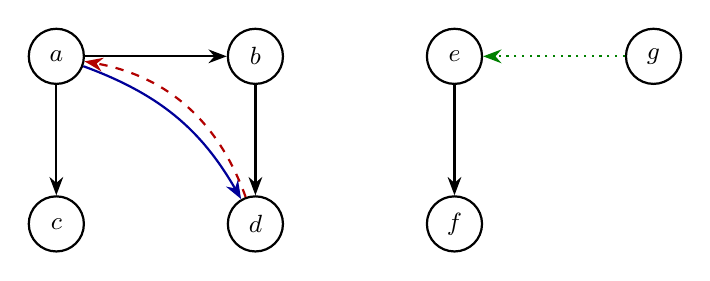
\begin{tikzpicture}[node distance=14mm]
    \node[vertex] (a) {$a$};
    \node[vertex, right=18mm of a] (b) {$b$};
    \node[vertex, below=14mm of a] (c) {$c$};
    \node[vertex, below=14mm of b] (d) {$d$};
    \node[vertex, right=18mm of b] (e) {$e$};
    \node[vertex, below=14mm of e] (f) {$f$};
    \node[vertex, right=18mm of e] (g) {$g$};
    % Tree edges
    \draw[treeedge] (a) -- (b);
    \draw[treeedge] (a) -- (c);
    \draw[treeedge] (b) -- (d);
    \draw[treeedge] (e) -- (f);
    % Back edge (d -> a, ancestor)
    \draw[backedge] (d) to[bend right=30] (a);
    % Forward edge (a -> d, descendant via longer tree path)
    \draw[fwdedge] (a) to[bend left=20] (d);
    % Cross edge (g -> e, separate DFS root)
    \draw[crossedge] (g) -- (e);
\end{tikzpicture}
\end{center}

\emph{DFS edge classification on a 7-vertex directed graph.}
DFS roots: $a$ first, then $e$, then $g$ (each picked when the
prior tree finishes). \emph{Tree edges} (solid black):
$a{\to}b$, $a{\to}c$, $b{\to}d$, $e{\to}f$ --- the parent-pointer
DFS tree. \emph{Back edge} (red dashed):
$d{\to}a$ closes the cycle $a{\to}b{\to}d{\to}a$.
\emph{Forward edge} (blue solid):
$a{\to}d$ skips ahead to a descendant via a non-tree edge.
\emph{Cross edge} (green dotted):
$g{\to}e$ jumps between separately rooted DFS trees and is
neither ancestor nor descendant of $g$.

In an \emph{undirected} graph, only tree edges and back edges
exist --- forward edges and cross edges collapse to back edges
under undirected DFS because every non-tree edge is examined
twice (once from each endpoint).

\subsection*{Cycle detection on directed graphs}

The classification gives a one-line directed-graph cycle test:
\textbf{a directed graph has a cycle if and only if directed-DFS
produces a back edge.} ``$\Leftarrow$'' is the back-edge
definition: $(u \to v)$ back edge means $v$ is an ancestor of
$u$, so $v \to \ldots \to u \to v$ is a cycle. ``$\Rightarrow$''
is harder: any cycle in $G$ produces a back edge during DFS,
because among the cycle's vertices the one with smallest discovery
time $d[\cdot]$ ends up an ancestor of the rest, and the
incoming-cycle-edge to that ancestor is a back edge.

In code, you don't need to maintain $d[\cdot] / f[\cdot]$
explicitly --- a tri-state \texttt{colour[]} array does the job.
A vertex is \textsc{white} (undiscovered), \textsc{gray} (on the
current DFS recursion stack, i.e.\ ``in progress''), or
\textsc{black} (finished). An edge $(u, v)$ to a \textsc{gray}
vertex \emph{is} a back edge.

\begin{lstlisting}[basicstyle=\ttfamily\small,frame=single]
enum Colour { WHITE, GRAY, BLACK };

bool hasCycleDFS(int u, const std::vector<std::vector<int>>& adj,
                 std::vector<Colour>& colour) {
    colour[u] = GRAY;
    for (int v : adj[u]) {
        if (colour[v] == GRAY) return true;          // back edge => cycle
        if (colour[v] == WHITE && hasCycleDFS(v, adj, colour))
            return true;
    }
    colour[u] = BLACK;
    return false;
}

bool hasCycle(const std::vector<std::vector<int>>& adj) {
    int n = adj.size();
    std::vector<Colour> colour(n, WHITE);
    for (int u = 0; u < n; ++u)
        if (colour[u] == WHITE && hasCycleDFS(u, adj, colour))
            return true;
    return false;
}
\end{lstlisting}

The outer loop over $u$ handles disconnected directed graphs ---
any vertex that has not yet been discovered launches a fresh DFS
tree. Cost is the same as plain DFS: $O(V + E)$.

\section{10.7 Directed Graphs}

\begin{defnbox}
\textbf{Directed graph (digraph).} Edges have direction. $(u \to v) \in E$ does \emph{not} imply $(v \to u) \in E$.

\textbf{Cycle.} A path that starts and ends at the same vertex.

\textbf{DAG (directed acyclic graph).} A directed graph with no cycles. The single most useful graph class in computer science.
\end{defnbox}

\subsection*{Why DAGs matter}

A DAG captures ``A must come before B'' relationships without contradicting itself. Anything that \emph{orders} things is a DAG:

\begin{itemize}[leftmargin=*]
    \item Course prerequisites ($\to$ topological sort).
    \item Build systems ($\to$ incremental rebuild).
    \item Spreadsheet formulas ($\to$ evaluation order).
    \item Git commit history ($\to$ merges and ancestors).
    \item Neural net forward passes.
    \item Dataflow programs.
\end{itemize}

If your directed graph has a cycle, you have a contradiction: A needs B first, but B also needs A first. Cycle detection on directed graphs is DFS plus a ``currently in recursion'' flag.

\subsection*{Representation}

Same adjacency list or matrix, but only one direction per edge:

\begin{lstlisting}[basicstyle=\ttfamily\small,frame=single]
// Directed: only add u -> v, not v -> u
adj[u].push_back(v);
\end{lstlisting}

\subsection*{Terminology that bites}

\begin{itemize}[leftmargin=*]
    \item \textbf{In-degree} of $v$: number of edges ending at $v$.
    \item \textbf{Out-degree} of $v$: number of edges starting at $v$.
    \item \textbf{Successor / predecessor}: $v$ is a successor of $u$ if $(u \to v) \in E$; then $u$ is a predecessor of $v$.
    \item \textbf{Source}: vertex with in-degree 0 (no one points to it).
    \item \textbf{Sink}: vertex with out-degree 0 (it points to no one).
\end{itemize}

\begin{examplebox}
\textbf{Kidney exchange as a cycle problem.} A directed edge $D \to R$ means ``donor family of patient $D$ is willing to give a kidney to recipient $R$.'' A $k$-way simultaneous exchange is a cycle of length $k$. Hospitals literally run cycle-detection algorithms on these graphs to match transplants -- a real-world optimization problem worth billions of dollars in life-years.
\end{examplebox}

\subsection*{The build-system DAG, drawn}

Every modern build system --- \texttt{make}, Bazel, Cargo, Ninja,
\texttt{cmake --build} --- is a topological sort of a dependency
DAG with a re-execution rule layered on top. Vertices are build
targets; an edge $u \to v$ means ``$v$ depends on $u$, so $u$
must be built before $v$.'' The topological order is a valid
build schedule, and any two vertices that aren't related by the
ancestor relation can be built in parallel. That last sentence is
exactly why \texttt{make -j8} works: independent subtrees of the
DAG are independent jobs.

\begin{center}
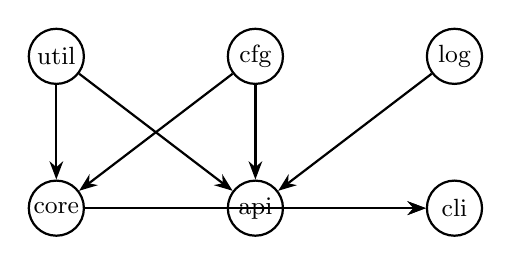
\begin{tikzpicture}[node distance=12mm and 18mm]
    \node[vertex] (util) {\small util};
    \node[vertex, right=of util] (cfg)  {\small cfg};
    \node[vertex, right=of cfg]  (log)  {\small log};
    \node[vertex, below=of util] (core) {\small core};
    \node[vertex, below=of cfg]  (api)  {\small api};
    \node[vertex, below=of log]  (cli)  {\small cli};
    \draw[edge] (util) -- (core);
    \draw[edge] (util) -- (api);
    \draw[edge] (cfg)  -- (api);
    \draw[edge] (cfg)  -- (core);
    \draw[edge] (log)  -- (api);
    \draw[edge] (core) -- (cli);
    \draw[edge] (api)  -- (cli);
\end{tikzpicture}
\end{center}

\emph{Six-target dependency DAG.}
A valid topological order is
\texttt{util}, \texttt{cfg}, \texttt{log}, \texttt{core},
\texttt{api}, \texttt{cli} --- but
\texttt{cfg}, \texttt{log}, \texttt{util}, \texttt{api},
\texttt{core}, \texttt{cli} works equally well. The first three
targets share no edges between them, so a parallel build invokes
their compilers concurrently; \texttt{cli} sits at the bottom and
must wait for both \texttt{core} and \texttt{api} to finish.
Add a cycle to this graph (say,
\texttt{cli} $\to$ \texttt{cfg} from a stray \texttt{\#include})
and \emph{no} build order exists --- which is exactly the error
modern build systems print.

\section{10.8 Weighted Graphs}

\begin{defnbox}
\textbf{Weighted graph.} Each edge carries a numerical weight (cost, distance, time, capacity, \ldots). Path length = sum of edge weights along the path.
\end{defnbox}

\subsection*{Why weights complicate things}

In an unweighted graph, ``shortest'' means ``fewest hops.'' BFS handles it. In a weighted graph, ``shortest'' means ``smallest total weight'' -- and a path with more edges can easily be shorter than one with fewer:

\begin{center}
A $\xrightarrow{10}$ C versus A $\xrightarrow{2}$ B $\xrightarrow{3}$ C  \quad (length 10 vs.\ 5)
\end{center}

BFS can't see this. You need an algorithm that explores in order of \emph{weighted distance}, not edge count -- enter Dijkstra (§10.9).

\subsection*{Representation}

\begin{lstlisting}[basicstyle=\ttfamily\small,frame=single]
// List form: (neighbor, weight) pairs.
std::vector<std::vector<std::pair<int,int>>> adj(V);
adj[u].emplace_back(v, w);

// Matrix form: INT_MAX (or INFINITY) marks "no edge".
std::vector<std::vector<int>> w(V, std::vector<int>(V, INT_MAX));
w[i][i] = 0;
w[u][v] = weight;
\end{lstlisting}

\subsection*{Negative weights}

Negative edge weights are allowed, but \textbf{negative cycles} break the shortest-path problem entirely: you can loop around the negative cycle forever, driving the total cost to $-\infty$. Shortest path is undefined.

\begin{warnbox}
\textbf{Dijkstra can't handle negative weights, period.} Its correctness proof relies on never having to revisit a ``finished'' vertex, and negative edges can make that false. Use Bellman-Ford (§10.10) or the special Johnson's algorithm if any edge is negative. Knowing which shortest-path algorithm tolerates which edge signs is a classic exam question.
\end{warnbox}

\subsection*{Relaxation: the universal SSSP primitive}

\begin{defnbox}
\textbf{Edge relaxation.} Given a weighted edge $(u, v, w)$ and
tentative distances $\texttt{dist}[\cdot]$, the \emph{relax} operation is

\begin{center}
\textbf{relax}$(u, v, w)$: \quad if $\texttt{dist}[u] + w < \texttt{dist}[v]$
then $\texttt{dist}[v] \gets \texttt{dist}[u] + w$,
$\texttt{prev}[v] \gets u$.
\end{center}

After \textsc{relax}$(u, v, w)$, $\texttt{dist}[v] \le \texttt{dist}[u] + w$
holds. The triangle inequality
$\texttt{dist}[v] \le \texttt{dist}[u] + w$ for every edge is the
\emph{shortest-path optimality condition} --- once it holds for all
edges, $\texttt{dist}[\cdot]$ records true shortest distances.
\end{defnbox}

Relaxation is monotonic: each call either decreases
$\texttt{dist}[v]$ or leaves it alone. Every single-source
shortest-path algorithm in this chapter --- DAG-relax, Dijkstra,
Bellman-Ford --- is just ``call \textsc{relax} on every edge in some
order; correctness comes from the order.'' The three differ only in
\emph{order}:

\begin{itemize}[leftmargin=*]
    \item \textbf{DAG-relax} (the easy case): topologically sort
          the DAG, then relax every outgoing edge of each vertex
          in topological order. One pass; $O(V + E)$.
          \emph{Correctness:} when we process $u$, any predecessor
          $p$ on the shortest $s \to v$ path has already been
          processed (it appears earlier in topological order), so
          $\texttt{dist}[u]$ is already final, and relaxing
          $(u, v, w)$ propagates the correct distance to $v$.
    \item \textbf{Dijkstra} (\S10.9): pick the unvisited vertex
          with smallest tentative distance and relax all its
          outgoing edges --- a greedy frontier expansion that
          works because non-negative edges guarantee
          $\texttt{dist}$-monotonic processing.
    \item \textbf{Bellman-Ford} (\S10.10): relax every edge
          $|V| - 1$ times. Slower but order-agnostic, so it
          tolerates negative weights and detects negative cycles.
\end{itemize}

Once you see the unification, picking the right algorithm collapses
to ``what's special about my edge weights / graph structure?''

\section{10.9 Dijkstra's Shortest Path}

\begin{ideabox}
\textbf{Dijkstra in one sentence.} BFS, but the frontier is a priority queue keyed by distance. Always expand the closest unvisited vertex next; its distance is now final.
\end{ideabox}

\subsection*{Algorithm}

For every vertex $v$, maintain:
\begin{itemize}[leftmargin=*]
    \item \texttt{dist[v]}: best-known shortest distance from the source (initially $\infty$).
    \item \texttt{prev[v]}: previous vertex along that best-known path (initially null).
\end{itemize}

At each step, pull the vertex with smallest tentative \texttt{dist} out of the priority queue (it won't improve), and \emph{relax} all its outgoing edges: for each edge $(u, v, w)$, if \texttt{dist[u] + w < dist[v]}, update \texttt{dist[v]} and \texttt{prev[v]}.

\begin{lstlisting}[basicstyle=\ttfamily\small,frame=single]
#include <queue>
#include <vector>
#include <limits>

using Edge = std::pair<int,int>;   // (neighbor, weight)
const int INF = std::numeric_limits<int>::max();

void dijkstra(const std::vector<std::vector<Edge>>& adj, int src,
              std::vector<int>& dist, std::vector<int>& prev) {
    int n = adj.size();
    dist.assign(n, INF);
    prev.assign(n, -1);
    dist[src] = 0;

    // Min-heap of (distance, vertex). std::greater flips the default max-heap.
    using PQE = std::pair<int,int>;
    std::priority_queue<PQE, std::vector<PQE>, std::greater<PQE>> pq;
    pq.push({0, src});

    while (!pq.empty()) {
        auto [d, u] = pq.top(); pq.pop();
        if (d > dist[u]) continue;          // stale entry -- already improved
        for (auto [v, w] : adj[u]) {
            int alt = d + w;
            if (alt < dist[v]) {
                dist[v] = alt;
                prev[v] = u;
                pq.push({alt, v});
            }
        }
    }
}
\end{lstlisting}

\begin{warnbox}
\textbf{The ``stale entry'' trick.} \texttt{std::priority\_queue} doesn't support decrease-key, so whenever we improve a vertex's distance, we just push a new, smaller entry. When we later pop, we check \texttt{if (d > dist[u]) continue;} to skip outdated entries. This is the idiomatic C++ Dijkstra -- simple, fast, and what you'd write in interviews or contests.
\end{warnbox}

\subsection*{Why it works -- greedy correctness}

\begin{ideabox}
When we pop the closest remaining vertex $u$ with tentative distance $d$, \emph{no later path can possibly be shorter}. Any other path to $u$ goes through some unvisited vertex $v$ with $\texttt{dist}[v] \geq d$ (that's why $u$ was chosen first), and then adds a non-negative edge weight on top of $\texttt{dist}[v]$, giving total $\geq d$. So $d$ is final at pop time. This is exactly why \textbf{Dijkstra requires non-negative edges}: the argument breaks if a negative edge can shave below $d$ after the fact.
\end{ideabox}

\subsection*{Negative-edge counterexample, drawn}

The cleanest illustration that Dijkstra can break on negative edges
is a 3-node graph:

\begin{center}
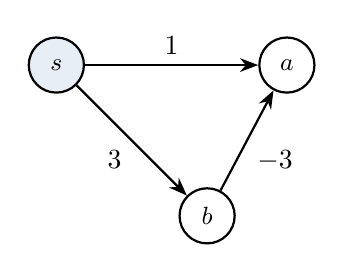
\begin{tikzpicture}[node distance=22mm]
    \node[vsource] (s) {$s$};
    \node[vertex, right=of s] (a) {$a$};
    \node[vertex, below right=14mm and 14mm of s] (b) {$b$};
    \draw[edge] (s) -- node[above] {$1$} (a);
    \draw[edge] (s) -- node[below left] {$3$} (b);
    \draw[edge] (b) -- node[below right] {$-3$} (a);
\end{tikzpicture}
\end{center}

True shortest distances from $s$: $\texttt{dist}[s] = 0$,
$\texttt{dist}[b] = 3$, $\texttt{dist}[a] = 0$ (via
$s \to b \to a$ at total $3 + (-3) = 0$).

What Dijkstra does, however: pop $s$ ($d = 0$), relax both edges so
$\texttt{dist}[a] = 1, \texttt{dist}[b] = 3$. Pop $a$ next (smallest
tentative $= 1$), declare $\texttt{dist}[a] = 1$ \emph{final}, finish
its empty out-list. Pop $b$, relax $b \to a$ with weight $-3$
finding $0 < 1$ --- but $a$ is already settled and we never
re-expand it. Dijkstra terminates with $\texttt{dist}[a] = 1$,
which is wrong by $1$.

The greedy-correctness proof above breaks at exactly the line
``adds a non-negative edge weight on top of $\texttt{dist}[v]$.''
With a negative edge, a later path \emph{can} undercut a
``finalised'' distance. Bellman-Ford (\S10.10) survives by relaxing
every edge $|V| - 1$ times instead of trusting a greedy ordering.

\subsection*{A worked Dijkstra trace}

\begin{center}
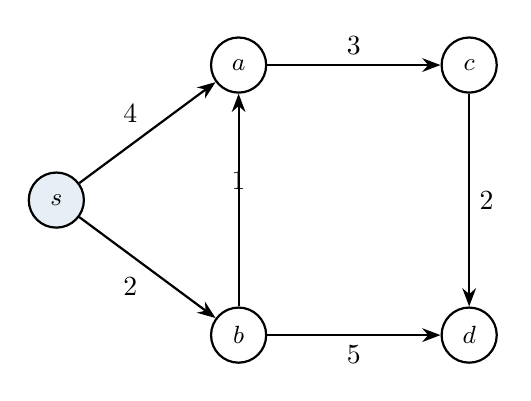
\begin{tikzpicture}[node distance=22mm]
    \node[vsource] (s) {$s$};
    \node[vertex, above right=12mm and 18mm of s] (a) {$a$};
    \node[vertex, below right=12mm and 18mm of s] (b) {$b$};
    \node[vertex, right=22mm of a] (c) {$c$};
    \node[vertex, right=22mm of b] (d) {$d$};
    \draw[edge] (s) -- node[above left] {$4$} (a);
    \draw[edge] (s) -- node[below left] {$2$} (b);
    \draw[edge] (a) -- node[above] {$3$} (c);
    \draw[edge] (b) -- node[above] {$1$} (a);
    \draw[edge] (b) -- node[below] {$5$} (d);
    \draw[edge] (c) -- node[right] {$2$} (d);
\end{tikzpicture}
\end{center}

\emph{5-node weighted directed graph.} Edge weights are all
non-negative, so Dijkstra is the right tool. Source is $s$.

\begin{examplebox}
\textbf{Dijkstra trace, frame by frame.} State at each step is
the priority queue (entries $(d, v)$, smallest-first) and the
$\texttt{dist}$ array. The $\infty$ symbol means ``not yet
relaxed.''

\medskip
\begin{tabular}{rp{6cm}|p{4.5cm}|l}
\hline
Step & action & PQ state & $\texttt{dist}[s,a,b,c,d]$ \\
\hline
0 & init & $[(0,s)]$ & $0, \infty, \infty, \infty, \infty$ \\
1 & pop $(0,s)$; relax $s{\to}a$ ($\infty\!\to\!4$), $s{\to}b$ ($\infty\!\to\!2$) & $[(2,b),(4,a)]$ & $0, 4, 2, \infty, \infty$ \\
2 & pop $(2,b)$; relax $b{\to}a$ ($4\!\to\!3$), $b{\to}d$ ($\infty\!\to\!7$) & $[(3,a),(4,a)^{*},(7,d)]$ & $0, 3, 2, \infty, 7$ \\
3 & pop $(3,a)$; relax $a{\to}c$ ($\infty\!\to\!6$) & $[(4,a)^{*},(6,c),(7,d)]$ & $0, 3, 2, 6, 7$ \\
4 & pop $(4,a)^{*}$; stale ($4 > \texttt{dist}[a] = 3$), skip & $[(6,c),(7,d)]$ & $0, 3, 2, 6, 7$ \\
5 & pop $(6,c)$; try $c{\to}d$: $6{+}2 = 8 \not< 7$, no-op & $[(7,d)]$ & $0, 3, 2, 6, 7$ \\
6 & pop $(7,d)$; no out-edges & $[\,]$ & $0, 3, 2, 6, 7$ \\
\hline
\end{tabular}

\medskip
Entries marked $(\cdot)^{*}$ are stale ones left in the heap by an
earlier improvement. Final $\texttt{dist} = [0, 3, 2, 6, 7]$.
Walking $\texttt{prev}[\cdot]$ back recovers each shortest path
--- e.g.\ $d \to b \to s$ at cost $7$.
\end{examplebox}

\begin{notebox}
\textbf{Decrease-key vs.\ lazy-deletion.} The textbook Dijkstra
calls \texttt{decrease-key} on the priority queue every time a
relaxation improves a vertex's tentative distance. With a binary
heap supporting \texttt{decrease-key} the cost is
$O((V + E) \log V)$ but the heap implementation needs an
\emph{index} that maps each vertex to its current heap slot ---
non-trivial. Standard libraries don't supply this; you'd reach for
\texttt{boost::heap::fibonacci\_heap} or roll your own indexed
binary heap to get textbook complexity.

The C++ idiom above (the ``stale-entry trick'') sidesteps the
problem: each relaxation pushes a \emph{new} smaller entry, leaving
the old larger entry in the heap as a tombstone. When a stale entry
surfaces at the top we detect it via \texttt{if (d > dist[u])
continue;} and discard. The asymptotic cost is the same
$O((V + E) \log V)$ for a binary heap because each edge produces at
most one heap push and the heap holds $O(E)$ entries; constants are
small and code is short. This is what production C++, competitive
programming, and most textbook references actually deploy ---
\texttt{decrease-key} is theoretically beautiful, lazy-deletion is
what ships.
\end{notebox}

\subsection*{Cost}

\begin{center}
\begin{tabular}{ll}
\hline
Priority-queue implementation & Runtime \\
\hline
Unsorted array / linear scan & $O(V^2 + E)$ \\
Binary heap (\texttt{std::priority\_queue}) & $O((V + E) \log V)$ \\
Fibonacci heap & $O(E + V \log V)$ \\
\hline
\end{tabular}
\end{center}

For sparse graphs, the binary-heap version is the sweet spot: simple, fast, what you'd reach for in real code. Fibonacci heaps have better theoretical bounds but rarely win in practice because of their hideous constant factors.

\subsection*{Reconstructing the path}

After Dijkstra, walk \texttt{prev} backwards from the destination:

\begin{lstlisting}[basicstyle=\ttfamily\small,frame=single]
std::vector<int> pathTo(int target, const std::vector<int>& prev) {
    std::vector<int> path;
    for (int v = target; v != -1; v = prev[v]) path.push_back(v);
    std::reverse(path.begin(), path.end());
    return path;
}
\end{lstlisting}

If \texttt{prev[target] == -1} and \texttt{target != src}, the target is unreachable.

\section{10.10 Bellman-Ford Shortest Path}

\begin{ideabox}
\textbf{Bellman-Ford in one sentence.} Relax every edge $V-1$ times. If any edge can \emph{still} be relaxed after that, there's a negative cycle. Slower than Dijkstra but handles negative weights.
\end{ideabox}

\subsection*{Algorithm}

\begin{lstlisting}[basicstyle=\ttfamily\small,frame=single]
struct Edge { int u, v, w; };

bool bellmanFord(int n, const std::vector<Edge>& edges, int src,
                 std::vector<int>& dist, std::vector<int>& prev) {
    dist.assign(n, INF);
    prev.assign(n, -1);
    dist[src] = 0;

    // Main loop: relax every edge V-1 times.
    for (int i = 0; i < n - 1; ++i) {
        for (const auto& e : edges) {
            if (dist[e.u] != INF && dist[e.u] + e.w < dist[e.v]) {
                dist[e.v] = dist[e.u] + e.w;
                prev[e.v] = e.u;
            }
        }
    }

    // Negative-cycle check: one more pass -- if anything still relaxes,
    // the graph has a reachable negative cycle.
    for (const auto& e : edges) {
        if (dist[e.u] != INF && dist[e.u] + e.w < dist[e.v])
            return false;
    }
    return true;
}
\end{lstlisting}

\subsection*{Why $V-1$ iterations?}

A shortest path has at most $V-1$ edges (any more would revisit a vertex, wasting weight if weights are non-negative -- and if weights are negative, see below). Each iteration propagates ``correct'' distances one edge farther along. After $V-1$ passes, every shortest path has been fully propagated, as long as no negative cycles exist.

If an edge is \emph{still} relaxable on a $V$-th iteration, then some path keeps getting shorter -- a negative cycle is the only way that can happen.

\begin{notebox}
\textbf{$|V|-1$-round correctness, by induction on path length.} Let
$\delta_k(v)$ denote the length of the shortest $s \to v$ path
\emph{using at most $k$ edges}. We show after the $k$-th outer
iteration $\texttt{dist}[v] \le \delta_k(v)$ for every $v$.

\emph{Base} ($k = 0$): only $s$ has a $0$-edge path, with cost $0$;
the initialisation $\texttt{dist}[s] = 0, \texttt{dist}[v] = \infty$
matches.

\emph{Step} ($k \to k{+}1$): a $(k{+}1)$-edge path to $v$ is some
$k$-edge path to a predecessor $p$ followed by edge $(p, v, w)$. By
IH $\texttt{dist}[p] \le \delta_k(p)$ after iteration $k$. The
$(k{+}1)$-th iteration relaxes \emph{every} edge, including
$(p, v, w)$, so afterwards
$\texttt{dist}[v] \le \texttt{dist}[p] + w \le \delta_k(p) + w
= \delta_{k+1}(v)$ (taking $p$ that achieves the minimum).

If the graph has no negative cycle, every shortest $s \to v$ path
is simple and uses at most $|V| - 1$ edges, so
$\delta_{|V|-1}(v) = \delta(v)$ (the true shortest-path cost). Thus
$|V| - 1$ iterations are enough.

If there \emph{is} a reachable negative cycle, there is some edge
$(u, v, w)$ on the cycle with
$\texttt{dist}[u] + w < \texttt{dist}[v]$ no matter how many rounds
we run; the $|V|$-th relaxation pass would still improve it. That's
the negative-cycle test: \emph{after} $|V| - 1$ rounds, do one
more --- any further relaxation $\Rightarrow$ negative cycle
reachable from $s$.
\end{notebox}

\subsection*{Cost}

$O(VE)$. Roughly $V$ times slower than Dijkstra in the worst case, but:

\begin{itemize}[leftmargin=*]
    \item Handles negative weights.
    \item Detects negative cycles.
    \item Works on \emph{any} graph representation -- just give it a list of edges.
    \item Easy to parallelize (independent edge relaxations).
\end{itemize}

\subsection*{Dijkstra vs.\ Bellman-Ford, decision flowchart}

\begin{center}
\begin{tabular}{lll}
\hline
Situation & Use \\
\hline
All edges non-negative, sparse & Dijkstra + binary heap \\
Negative edges, no negative cycles & Bellman-Ford \\
Need to detect negative cycles & Bellman-Ford \\
All-pairs shortest paths & Floyd-Warshall (§10.13) \\
Unweighted graph & BFS (not either of these) \\
\hline
\end{tabular}
\end{center}

\begin{notebox}
\textbf{SPFA} (``Shortest Path Faster Algorithm'') is a queue-based refinement of Bellman-Ford that's often faster in practice -- only re-process vertices whose distance actually changed. Worst case is still $O(VE)$, but average behavior on real graphs is much better.
\end{notebox}

\begin{examplebox}
\textbf{Bellman-Ford trace, with negative-cycle case.} Edge list
$E = [(s, a, 4), (s, b, 5), (a, c, -3), (b, c, 1), (c, b, -2)]$
on 4 vertices $\{s, a, b, c\}$, source $s$. Walk the relaxations
in the listed edge order each pass; show $\texttt{dist}$ after
each full pass.

\medskip
\begin{tabular}{rp{8.5cm}|l}
\hline
Pass & relaxations & $\texttt{dist}[s, a, b, c]$ \\
\hline
0 & init & $0, \infty, \infty, \infty$ \\
1 & $s{\to}a$ ($\infty\!\to\!4$), $s{\to}b$ ($\infty\!\to\!5$),
    $a{\to}c$ ($\infty\!\to\!1$), $c{\to}b$ ($5\!\to\!-1$). & $0, 4, -1, 1$ \\
2 & $b{\to}c$ ($1\!\to\!0$), $c{\to}b$ ($-1\!\to\!-2$). & $0, 4, -2, 0$ \\
3 & $b{\to}c$ ($0\!\to\!-1$), $c{\to}b$ ($-2\!\to\!-3$). & $0, 4, -3, -1$ \\
\hline
$|V|{-}1 = 3$ rounds done, but \dots & & \\
\hline
4 & $b{\to}c$ relaxes $-3 + 1 = -2 < -1$ $\Rightarrow$ negative cycle. & --- \\
\hline
\end{tabular}

\medskip
The cycle is $b \to c \to b$ with weight $1 + (-2) = -1 < 0$, so
each pass over $\{b, c\}$ shaves another $-1$ off both distances
indefinitely. Bellman-Ford's $|V|$-th-round test catches it ---
the algorithm returns \texttt{false} and the caller knows
shortest paths from $s$ to $\{b, c\}$ are undefined.

\smallskip
If we delete the $c \to b$ edge (no negative cycle, just one
negative edge $a \to c$ with weight $-3$), Bellman-Ford
converges to $\texttt{dist} = [0, 4, 5, 1]$ after one full pass
and the $|V|$-th-round test reports no further relaxation.
Negative edges alone are fine; negative \emph{cycles reachable
from the source} are not.
\end{examplebox}

\section{10.11 Topological Sort}

\begin{defnbox}
\textbf{Topological sort.} A linear ordering of a DAG's vertices such that every edge $u \to v$ has $u$ appearing before $v$. Exists iff the graph is acyclic. Not unique: most DAGs have many valid orderings.
\end{defnbox}

\begin{ideabox}
\textbf{The canonical use case.} Whenever you have ``do A before B'' constraints and want a valid linear schedule, you want topological sort. Course prerequisites, build orders, spreadsheet evaluation, task scheduling, dataflow execution -- all the same problem.
\end{ideabox}

\subsection*{Kahn's algorithm (in-degree method)}

Repeatedly peel off vertices with no incoming edges -- they're safe to do first.

\begin{lstlisting}[basicstyle=\ttfamily\small,frame=single]
std::vector<int> topoSortKahn(int n,
                              const std::vector<std::vector<int>>& adj) {
    std::vector<int> indeg(n, 0);
    for (int u = 0; u < n; ++u)
        for (int v : adj[u]) ++indeg[v];

    std::queue<int> q;
    for (int u = 0; u < n; ++u)
        if (indeg[u] == 0) q.push(u);

    std::vector<int> order;
    while (!q.empty()) {
        int u = q.front(); q.pop();
        order.push_back(u);
        for (int v : adj[u])
            if (--indeg[v] == 0) q.push(v);
    }

    if ((int)order.size() != n) return {};  // cycle detected
    return order;
}
\end{lstlisting}

If the final order doesn't have all $n$ vertices, the remaining vertices form a cycle -- automatic cycle detection, no extra work.

\subsection*{DFS-based topological sort}

Alternative: DFS, and \emph{push each vertex onto a result stack when it finishes} (after its recursion returns). Reverse the stack.

\begin{lstlisting}[basicstyle=\ttfamily\small,frame=single]
void dfsTopo(int u, const std::vector<std::vector<int>>& adj,
             std::vector<bool>& visited, std::vector<int>& out) {
    visited[u] = true;
    for (int v : adj[u])
        if (!visited[v]) dfsTopo(v, adj, visited, out);
    out.push_back(u);   // post-order: u is "done" now
}

std::vector<int> topoSortDfs(int n,
                             const std::vector<std::vector<int>>& adj) {
    std::vector<bool> visited(n, false);
    std::vector<int> out;
    for (int u = 0; u < n; ++u)
        if (!visited[u]) dfsTopo(u, adj, visited, out);
    std::reverse(out.begin(), out.end());
    return out;
}
\end{lstlisting}

Why the reversal? DFS finishes deeper-in-the-dependency-chain vertices first. In a topological ordering, those should come \emph{last} (they depend on earlier stuff). Reversing puts them in the right order.

\subsection*{Cost}

Both are $O(V + E)$.

\subsection*{Kahn vs.\ DFS}

\begin{itemize}[leftmargin=*]
    \item \textbf{Kahn} is iterative and natural for streaming/parallel processing -- multiple vertices can be in the ``ready'' queue simultaneously.
    \item \textbf{DFS} is shorter to write and fits naturally with other DFS-based algorithms (SCC, cycle detection).
\end{itemize}

Pick based on context. Most textbooks teach DFS; most real-world schedulers (like Tarjan's, or \texttt{make}'s job dispatcher) use Kahn-style because they can work on ``what's ready now'' incrementally.

\begin{notebox}
\textbf{Connection to \S10.6 edge classification.} The DFS-based
topological sort and the \S10.6 directed-cycle detector are the
\emph{same DFS}, read off two different ways. A directed graph has a
topological order $\Leftrightarrow$ it has no cycle
$\Leftrightarrow$ DFS produces no back edge. The
\texttt{dfsTopo} body above is a back-edge-free DFS that emits its
post-order; if a back edge \emph{did} appear, the post-order
reversal wouldn't be a valid topological order (we'd see a
descendant before its ancestor). Production implementations weave
the two together: a single DFS pass that emits the post-order
\emph{and} reports any back edge as ``cycle detected, no topo
order'' --- one tri-state \texttt{colour[]} array, one traversal,
both answers.
\end{notebox}

\section{10.12 Minimum Spanning Tree}

\begin{defnbox}
\textbf{Spanning tree.} A subset of a connected graph's edges that connects all vertices and forms a tree ($V-1$ edges, no cycles).

\textbf{Minimum spanning tree (MST).} A spanning tree with the smallest possible sum of edge weights. Requires a connected, undirected, weighted graph.
\end{defnbox}

\begin{examplebox}
\textbf{Physical intuition.} You're the electric company. Each edge is a potential power line between two cities, with a cost (length, terrain difficulty). You must connect every city. What's the cheapest wiring plan? That's an MST.
\end{examplebox}

\subsection*{Kruskal's algorithm (greedy edges)}

Sort all edges by weight. Add each edge to the MST unless it would create a cycle. Stop when you have $V-1$ edges.

``Would it create a cycle?'' is answered with a \textbf{union-find} (disjoint-set) data structure: two vertices are in the same component iff their roots are equal.

\begin{lstlisting}[basicstyle=\ttfamily\small,frame=single]
struct DSU {
    std::vector<int> parent, rank_;
    DSU(int n) : parent(n), rank_(n, 0) {
        std::iota(parent.begin(), parent.end(), 0);
    }
    int find(int x) {
        while (parent[x] != x) {
            parent[x] = parent[parent[x]];   // path compression
            x = parent[x];
        }
        return x;
    }
    bool unite(int a, int b) {
        a = find(a); b = find(b);
        if (a == b) return false;
        if (rank_[a] < rank_[b]) std::swap(a, b);
        parent[b] = a;
        if (rank_[a] == rank_[b]) ++rank_[a];
        return true;
    }
};

struct Edge { int u, v, w; };

std::vector<Edge> kruskal(int n, std::vector<Edge> edges) {
    std::sort(edges.begin(), edges.end(),
              [](const Edge& a, const Edge& b){ return a.w < b.w; });

    DSU dsu(n);
    std::vector<Edge> mst;
    for (const auto& e : edges) {
        if (dsu.unite(e.u, e.v)) {
            mst.push_back(e);
            if ((int)mst.size() == n - 1) break;
        }
    }
    return mst;
}
\end{lstlisting}

\subsection*{Cost}

$O(E \log E) = O(E \log V)$ (since $E \leq V^2$, the two are equivalent up to a constant factor). Dominated by the sort; union-find operations are near-$O(1)$ amortized.

\subsection*{Why the greedy works}

\begin{defnbox}
\textbf{Cut property.} A \emph{cut} of a connected undirected graph
$G = (V, E)$ is a partition $V = S \sqcup (V \setminus S)$ with
$S \neq \emptyset, V$. An edge $(u, v)$ \emph{crosses} the cut if
$u \in S$ and $v \in V \setminus S$ (or vice versa). The cut
property says: for any cut whose crossing edges have a unique
minimum-weight edge $e^* = (u^*, v^*, w^*)$, every MST of $G$
contains $e^*$. (With ties, $e^*$ is in \emph{some} MST.)

\emph{Sketched proof (exchange argument).} Take any MST $T$. If
$T$ contains $e^*$, done. Otherwise $T \cup \{e^*\}$ has a cycle
$C$ that uses $e^*$ plus other edges; $C$ must cross the cut an
even number of times, so $C$ contains another crossing edge
$e' = (u', v', w')$ with $w' > w^*$. Then
$T' = T \cup \{e^*\} \setminus \{e'\}$ is a spanning tree with
total weight $w(T) - w' + w^* < w(T)$, contradicting $T$ being
minimum. So $e^* \in T$ after all. (CLRS Theorem 23.1.)
\end{defnbox}

\begin{defnbox}
\textbf{Cycle property.} For any cycle $C$ in $G$, the
unique-maximum-weight edge of $C$ is in \emph{no} MST. (With ties,
no MST is forced to contain any specific maximum-weight edge of
$C$.)

\emph{Sketched proof.} Suppose some MST $T$ contains a unique
max-weight edge $e^* = (u^*, v^*, w^*)$ of $C$. Removing $e^*$
splits $T$ into two components $S, V \setminus S$. Since $C$ is a
cycle through $e^*$, $C$ contains another edge $e'$ crossing the
cut $(S, V \setminus S)$ with $w' < w^*$. Then
$T' = T \cup \{e'\} \setminus \{e^*\}$ is a spanning tree of
strictly smaller total weight, contradicting MST-minimality. (CLRS
Theorem 23.2.)
\end{defnbox}

These two lemmas justify both Kruskal and Prim:
\begin{itemize}[leftmargin=*]
    \item \textbf{Kruskal.} Each \texttt{unite}-accepting edge is
          the minimum-weight edge across the cut
          $(S, V \setminus S)$ where $S$ is the connected component
          of $u$ in the partial MST. So by the cut property the edge
          is safe to take.
    \item \textbf{Prim.} Each ``cheapest edge from the inside set
          to an outside vertex'' is the minimum-weight edge across
          the cut $(\text{inside}, \text{outside})$. Same cut
          property, different cut.
\end{itemize}

The cycle property is the \emph{anti}-MST companion: it tells you
which edges to never bother with --- whenever a cycle's heaviest
edge can be replaced by a lighter cycle alternative, the heavy edge
is dead weight.

\subsection*{Prim's algorithm (greedy vertex frontier)}

Alternative MST algorithm: start from any vertex, repeatedly add
the cheapest edge that connects an ``inside'' vertex to an
``outside'' vertex. Structurally it's Dijkstra with a different
relaxation rule --- compare \emph{edge weight directly}, not
cumulative distance. The min-heap holds (edge weight, outside
vertex, inside parent) tuples; we pop the cheapest crossing edge,
add the outside vertex to the inside set, and push the
newly-uncovered edges.

\begin{lstlisting}[basicstyle=\ttfamily\small,frame=single]
struct PrimEdge { int w, v, parent; };
struct PrimCmp {
    bool operator()(const PrimEdge& a, const PrimEdge& b) const {
        return a.w > b.w;   // min-heap on weight
    }
};

// adj[u] = vector of (neighbour, weight) pairs.
std::vector<Edge> prim(int n,
                       const std::vector<std::vector<std::pair<int,int>>>& adj) {
    std::vector<bool> inMST(n, false);
    std::priority_queue<PrimEdge, std::vector<PrimEdge>, PrimCmp> pq;
    pq.push({0, 0, -1});                          // start at vertex 0

    std::vector<Edge> mst;
    while (!pq.empty() && (int)mst.size() < n - 1) {
        auto [w, v, parent] = pq.top(); pq.pop();
        if (inMST[v]) continue;                   // stale entry, skip
        inMST[v] = true;
        if (parent != -1)
            mst.push_back({parent, v, w});
        for (auto [nbr, weight] : adj[v])
            if (!inMST[nbr])
                pq.push({weight, nbr, v});
    }
    return mst;                                   // empty if graph disconnected
}
\end{lstlisting}

The same \emph{stale-entry / lazy-deletion} idiom from \S10.9
Dijkstra applies: we push duplicates instead of decrease-key, and
filter by \texttt{inMST[v]} on pop. With a binary heap the cost is
$O((V + E) \log V)$. With an array-based priority queue and
$O(V)$ extract-min the cost is $O(V^2)$ --- and on a dense graph
($E = \Theta(V^2)$) array-Prim's $O(V^2)$ \emph{beats} Kruskal's
$O(E \log E) = O(V^2 \log V)$ because we skip the sort and the
union-find both. Production graph libraries pick by density.

\begin{center}
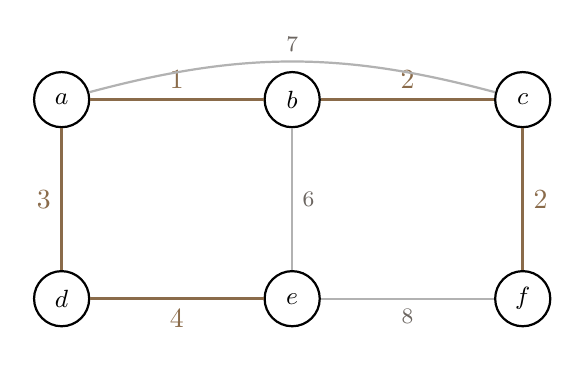
\begin{tikzpicture}[node distance=18mm and 22mm]
    \node[vertex] (a) {$a$};
    \node[vertex, right=of a] (b) {$b$};
    \node[vertex, right=of b] (c) {$c$};
    \node[vertex, below=of a] (d) {$d$};
    \node[vertex, below=of b] (e) {$e$};
    \node[vertex, below=of c] (f) {$f$};
    % MST edges (heavy)
    \draw[mstedge] (a) -- node[above] {$1$} (b);
    \draw[mstedge] (b) -- node[above] {$2$} (c);
    \draw[mstedge] (a) -- node[left]  {$3$} (d);
    \draw[mstedge] (d) -- node[below] {$4$} (e);
    \draw[mstedge] (c) -- node[right] {$2$} (f);
    % Non-MST edges (thin grey)
    \draw[uedge, gray!60] (b) -- node[right, mutedtext, font=\footnotesize] {$6$} (e);
    \draw[uedge, gray!60] (e) -- node[below, mutedtext, font=\footnotesize] {$8$} (f);
    \draw[uedge, gray!60] (a) to[bend left=15] node[above, mutedtext, font=\footnotesize] {$7$} (c);
\end{tikzpicture}
\end{center}

\emph{6-vertex weighted graph and its MST.} Heavy tan edges form
the MST (total weight $1{+}2{+}3{+}4{+}2 = 12$), thin grey edges
are the non-MST edges $(b,e,6), (e,f,8), (a,c,7)$. Cut-property
sanity check on the cut
$S = \{a\}, V \setminus S = \{b, c, d, e, f\}$: crossing edges are
$(a,b,1), (a,d,3), (a,c,7)$, with min $(a,b,1)$ --- which is in the
MST. By the cycle property, the cycle
$a{-}b{-}c{-}a$ (weights $1, 2, 7$) has heaviest edge $(a,c,7)$,
which is correctly excluded.

\begin{notebox}
\textbf{DSU's amortised cost: $O(\alpha(n))$ via inverse Ackermann.}
The Kruskal \texttt{DSU} above implements both path compression
(\texttt{parent[x] = parent[parent[x]]} as we walk up) and
union-by-rank (lower-rank tree gets reattached under the
higher-rank one). With both, a sequence of $m$ \texttt{find} +
\texttt{unite} operations costs
$O(m \cdot \alpha(n))$ amortised, where $\alpha(\cdot)$ is the
inverse Ackermann function. For $n \le 2^{2^{2^{16}}}$
(astronomically more atoms than the observable universe contains),
$\alpha(n) \le 4$, so each operation is effectively $O(1)$ in any
realistic setting.

The proof is genuinely hard --- Tarjan's 1975 paper introduced the
amortised-analysis framework that ch.~9 \S9.9 augmentation-cost
arguments use. CLRS Ch~21 carries the full derivation. For us, the
operative fact is: $\alpha(n)$ never exceeds $4$ in practice, so
Kruskal's runtime in the wild is dominated by the
$O(E \log E)$ sort, not the union-find.
\end{notebox}

\begin{center}
\begin{tabular}{lll}
\hline
& Kruskal & Prim \\
\hline
Approach & greedy on edges & greedy on vertex frontier \\
Needs & sorted edge list, union-find & adjacency list, priority queue \\
Cost & $O(E \log E)$ & $O(E \log V)$ w/ binary heap \\
Good when & edges are easy to enumerate & graph is dense, adjacency is fast \\
\hline
\end{tabular}
\end{center}

\begin{notebox}
For a dense graph ($E = \Theta(V^2)$), Prim with an array-based priority queue runs in $O(V^2)$, which beats Kruskal's $O(V^2 \log V)$. For sparse graphs, they're essentially tied.
\end{notebox}

\section{10.13 All-Pairs Shortest Path (Floyd-Warshall)}

\begin{ideabox}
\textbf{Floyd-Warshall in one sentence.} Compute shortest path from \emph{every} vertex to every other vertex by, in turn, allowing each vertex as an intermediate step. Three nested loops, no priority queue, $O(V^3)$.
\end{ideabox}

\subsection*{Algorithm}

Maintain \texttt{dist[i][j]} = current best-known distance from $i$ to $j$. Initialize:
\begin{itemize}[leftmargin=*]
    \item \texttt{dist[i][i] = 0}.
    \item \texttt{dist[i][j] = w(i,j)} if the edge exists.
    \item \texttt{dist[i][j] = $\infty$} otherwise.
\end{itemize}

Then iterate: for each intermediate vertex $k$, for each pair $(i, j)$, ask ``does going through $k$ beat the current best?''

\begin{lstlisting}[basicstyle=\ttfamily\small,frame=single]
void floydWarshall(std::vector<std::vector<int>>& dist) {
    int n = dist.size();
    for (int k = 0; k < n; ++k)
        for (int i = 0; i < n; ++i)
            for (int j = 0; j < n; ++j)
                if (dist[i][k] != INF && dist[k][j] != INF
                    && dist[i][k] + dist[k][j] < dist[i][j])
                    dist[i][j] = dist[i][k] + dist[k][j];
}
\end{lstlisting}

\subsection*{Why it works -- the $k$-loop invariant}

\begin{ideabox}
After the $k$-th outer iteration, \texttt{dist[i][j]} is the shortest path from $i$ to $j$ using \emph{only vertices $\{0, 1, \ldots, k\}$ as intermediates}. When $k = n-1$, that's the shortest path using any vertex, which is the answer. The $k$ loop must be \emph{outermost} -- swapping the loop order breaks the invariant and gives wrong answers. This is a favorite homework trap.
\end{ideabox}

\subsection*{Cost}

$O(V^3)$ time, $O(V^2)$ space. That's cubic, but with tiny constants -- three nested for loops of integer additions. On modern hardware it's vectorizable and absolutely flies for $V$ up to a few thousand.

\subsection*{Floyd-Warshall vs.\ running Dijkstra $V$ times}

\begin{center}
\begin{tabular}{lll}
\hline
& Dijkstra from every source & Floyd-Warshall \\
\hline
Total cost (binary heap) & $O(V (V+E) \log V)$ & $O(V^3)$ \\
Handles negative edges? & no & yes \\
Detects negative cycles? & no & yes (check diagonal) \\
Code complexity & moderate & very simple \\
Ideal on & sparse, non-negative & dense, or need negative-weight support \\
\hline
\end{tabular}
\end{center}

\begin{warnbox}
\textbf{Negative cycle detection.} After Floyd-Warshall, if any \texttt{dist[i][i] < 0}, there's a negative cycle through vertex $i$. Slick -- no extra pass needed.
\end{warnbox}

\subsection*{Path reconstruction}

Floyd-Warshall only computes distances. To recover paths, track the intermediate vertex alongside:

\begin{lstlisting}[basicstyle=\ttfamily\small,frame=single]
std::vector<std::vector<int>> next;   // next[i][j] = first hop from i toward j

// During init: next[i][j] = j if edge exists, else -1; next[i][i] = i.
// During update:
if (dist[i][k] + dist[k][j] < dist[i][j]) {
    dist[i][j] = dist[i][k] + dist[k][j];
    next[i][j] = next[i][k];
}

// Reconstruct path i -> j:
std::vector<int> path = {i};
while (path.back() != j) path.push_back(next[path.back()][j]);
\end{lstlisting}

\subsection*{Algebraic view}

Floyd-Warshall is min-plus matrix multiplication in disguise. Replace ``product + sum'' with ``sum + min,'' and the adjacency matrix raised to high enough a power (in this semiring) is exactly the all-pairs-shortest-path matrix. This connects shortest paths to a whole field of tropical algebra, used in everything from compiler optimization to network calculus.

\begin{notebox}
\textbf{Floyd-Warshall as relaxation, restated.} The
\texttt{dist[i][j] = min(dist[i][j], dist[i][k] + dist[k][j])}
update is exactly an edge relaxation in the meta-graph whose
``edges'' are existing best-known $(i, j)$-paths and whose
relaxation key is ``allow $k$ as a new intermediate.'' DAG-relax
relaxes per topological vertex, Dijkstra relaxes per
distance-monotonic vertex, Bellman-Ford relaxes per pass,
Floyd-Warshall relaxes per intermediate vertex. The four are the
same primitive applied with four different orderings of edge
relaxations --- the unification \S10.8 promised, now closed at the
chapter's last algorithm.
\end{notebox}

\section{10.14 Strongly Connected Components}

\begin{defnbox}
\textbf{Strongly connected component (SCC).} In a directed graph
$G = (V, E)$, two vertices $u, v$ are \emph{strongly connected}
if there is a path $u \to v$ \emph{and} a path $v \to u$. Strong
connectivity is an equivalence relation; its equivalence classes
are the SCCs. Each SCC is a maximal set of mutually reachable
vertices.

\textbf{Condensation graph.} Contract each SCC to a single
vertex. The result is always a \emph{DAG} --- the SCC-DAG of $G$
--- because any cycle among contracted vertices would have merged
them into one SCC.
\end{defnbox}

\begin{ideabox}
SCC-decomposition is the universal preprocessing step for every
``directed-graph reachability'' problem. After computing SCCs you
work with the SCC-DAG and run any DAG algorithm
(topological sort, DAG shortest paths, dynamic programming) on the
condensation. Cycles in the original graph become single
``super-vertices'' in the DAG; the DAG carries all the inter-cycle
structure.
\end{ideabox}

\subsection*{Kosaraju's algorithm (DFS twice)}

The trick is to combine \S10.6's DFS finish-time ordering with the
\emph{transpose} graph $G^T$ (every edge reversed). Two passes:

\begin{enumerate}
    \item Run DFS on $G$ and push vertices to a stack \emph{in
          finish-time order} (the latest-finishing vertex on top).
    \item Pop vertices off the stack one at a time. Each pop runs
          a fresh DFS \emph{in $G^T$} starting at the popped
          vertex, restricted to so-far-unvisited vertices. The set
          of vertices each restricted DFS reaches is one SCC.
\end{enumerate}

\emph{Why it works:} the latest-finishing vertex of pass 1 is in a
``source SCC'' of the SCC-DAG (no incoming inter-SCC edges). DFS
from that vertex in $G^T$ reverses the inter-SCC edges, so it
\emph{cannot} escape its own SCC --- giving exactly the SCC's
vertex set. Removing those, the next latest-finishing unvisited
vertex is in the next source SCC of the remaining DAG, and so on.
CLRS Theorem 22.16 carries the proof.

\begin{lstlisting}[basicstyle=\ttfamily\small,frame=single]
// Pass 1: DFS on G, pushing vertices in finish-time order.
void dfsForward(int u, const std::vector<std::vector<int>>& adj,
                std::vector<bool>& visited, std::vector<int>& order) {
    visited[u] = true;
    for (int v : adj[u])
        if (!visited[v]) dfsForward(v, adj, visited, order);
    order.push_back(u);   // post-order: latest finishes go on the back
}

// Pass 2: DFS on G^T, collecting one SCC per call.
void dfsBackward(int u, const std::vector<std::vector<int>>& adjT,
                 std::vector<bool>& assigned, std::vector<int>& comp) {
    assigned[u] = true;
    comp.push_back(u);
    for (int v : adjT[u])
        if (!assigned[v]) dfsBackward(v, adjT, assigned, comp);
}

std::vector<std::vector<int>> kosaraju(
        int n, const std::vector<std::vector<int>>& adj) {
    // Build transpose G^T.
    std::vector<std::vector<int>> adjT(n);
    for (int u = 0; u < n; ++u)
        for (int v : adj[u]) adjT[v].push_back(u);

    // Pass 1.
    std::vector<bool> visited(n, false);
    std::vector<int> order;
    for (int u = 0; u < n; ++u)
        if (!visited[u]) dfsForward(u, adj, visited, order);

    // Pass 2: pop vertices in reverse finish order, DFS on G^T.
    std::vector<bool> assigned(n, false);
    std::vector<std::vector<int>> sccs;
    for (int i = (int)order.size() - 1; i >= 0; --i) {
        int u = order[i];
        if (!assigned[u]) {
            std::vector<int> comp;
            dfsBackward(u, adjT, assigned, comp);
            sccs.push_back(std::move(comp));
        }
    }
    return sccs;
}
\end{lstlisting}

Cost is $O(V + E)$: two linear-time DFS traversals plus one
transpose construction. Output \texttt{sccs} is a list of vertex
sets, one per SCC, emitted in topological order on the SCC-DAG (the
first SCC popped is a source).

\begin{notebox}
\textbf{Tarjan's algorithm} computes SCCs in a \emph{single} DFS
pass using two augmentations per vertex --- \texttt{disc[u]}
(discovery time) and \texttt{low[u]} (smallest \texttt{disc}
reachable via tree edges plus at most one back edge from $u$'s
subtree). When DFS finishes a vertex $u$ with
$\texttt{disc[u]} = \texttt{low[u]}$, $u$ is the root of its SCC,
and that SCC is exactly the contiguous span of an explicit DFS
stack popped down to $u$. Same $O(V + E)$ asymptotic cost, half the
constant factor (no transpose to build), but the correctness
argument is more delicate. Use Tarjan when constant factors matter
or you can't afford the $O(E)$ transpose memory; use Kosaraju when
clarity wins. CLRS \S22.5 has Kosaraju; the Tarjan derivation lives
in CLRS exercises and Sedgewick \S4.2.
\end{notebox}

\begin{center}
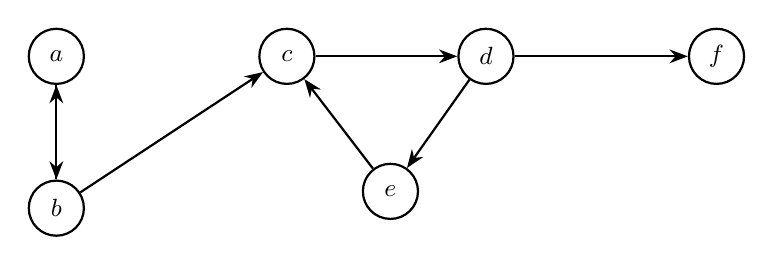
\begin{tikzpicture}[node distance=12mm and 18mm]
    % SCC 1: {a, b}
    \node[vertex] (a) {$a$};
    \node[vertex, below=of a] (b) {$b$};
    % SCC 2: {c, d, e}
    \node[vertex, right=22mm of a] (c) {$c$};
    \node[vertex, right=of c] (d) {$d$};
    \node[vertex, below right=12mm and 8mm of c] (e) {$e$};
    % SCC 3: {f}
    \node[vertex, right=22mm of d] (f) {$f$};
    \draw[edge] (a) -- (b);
    \draw[edge] (b) -- (a);
    \draw[edge] (b) -- (c);
    \draw[edge] (c) -- (d);
    \draw[edge] (d) -- (e);
    \draw[edge] (e) -- (c);
    \draw[edge] (d) -- (f);
\end{tikzpicture}

\medskip
\emph{Three SCCs in this 6-vertex digraph.} $\{a, b\}$ via the
$a \leftrightarrow b$ pair; $\{c, d, e\}$ via the cycle
$c \to d \to e \to c$; $\{f\}$ singleton. Inter-SCC edges
$b \to c$ and $d \to f$ collapse to a 3-vertex condensation DAG
$\{a,b\} \to \{c,d,e\} \to \{f\}$.

\smallskip
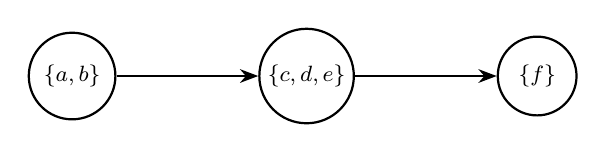
\begin{tikzpicture}[node distance=18mm]
    \node[vertex, minimum size=11mm, font=\footnotesize] (S1) {$\{a,b\}$};
    \node[vertex, minimum size=12mm, font=\footnotesize, right=of S1] (S2) {$\{c,d,e\}$};
    \node[vertex, minimum size=10mm, font=\footnotesize, right=of S2] (S3) {$\{f\}$};
    \draw[edge] (S1) -- (S2);
    \draw[edge] (S2) -- (S3);
\end{tikzpicture}
\end{center}

\subsection*{Applications}

SCCs are the workhorse for two production-relevant problems:

\begin{itemize}[leftmargin=*]
    \item \textbf{2-SAT solving in linear time.} Encode a 2-SAT
          formula $\bigwedge_i (\ell_i \vee \ell'_i)$ as the
          \emph{implication graph} on $2n$ literals: each clause
          $(\ell \vee \ell')$ contributes two edges,
          $\neg \ell \to \ell'$ and $\neg \ell' \to \ell$.
          The formula is satisfiable iff no variable $x$ has $x$
          and $\neg x$ in the \emph{same} SCC --- and a satisfying
          assignment is recovered from the SCC topological order.
          Total cost $O(n + m)$. Compare 3-SAT, which is
          NP-complete --- the SCC decomposition is what makes
          2-SAT tractable.
    \item \textbf{Dependency-cycle detection in package
          managers.} \texttt{cargo}, \texttt{npm}, \texttt{pip}
          all need to detect when a set of packages forms a
          mutual-dependency cycle (which prevents a clean install
          order). SCC computation surfaces every such cycle as a
          non-singleton SCC; the package manager either errors
          out or treats the SCC as a single ``compile-everyone-
          together'' unit, depending on the language's circular-
          import rules.
\end{itemize}

\section{10.15 Picking the right algorithm: master decision table}

By now you've seen seven (sometimes eight) graph algorithms with
overlapping use-cases. The right tool depends on \emph{which
problem} (single-pair / single-source / all-pairs / MST /
topological / cycle-detect / SCC / connectivity) and \emph{which
graph properties} (unweighted / non-negative / negative-no-cycle /
negative-with-cycle / DAG / sparse / dense). The following master
chooser collapses every chapter algorithm into one place. Cell
entries name the algorithm, complexity, and chapter section.

\begin{center}
\renewcommand{\arraystretch}{1.2}
\footnotesize
\noindent\resizebox{\textwidth}{!}{%
\begin{tabular}{p{3.2cm}|p{2.9cm}|p{3.2cm}|p{3.6cm}|p{2.6cm}}
\hline
\textbf{Problem $\downarrow$\ /\ Graph $\rightarrow$}
& \textbf{Unweighted / unit edges}
& \textbf{Non-negative weights}
& \textbf{Negative weights, no negative cycle}
& \textbf{DAG} \\
\hline
Single-source shortest path
& BFS, $O(V{+}E)$, \S10.5
& Dijkstra, $O((V{+}E)\log V)$, \S10.9
& Bellman-Ford, $O(VE)$, \S10.10
& DAG-relax, $O(V{+}E)$, \S10.8 \\
\hline
Single-pair shortest path
& BFS, $O(V{+}E)$, \S10.5
& Dijkstra (early-exit on target), \S10.9
& Bellman-Ford, \S10.10
& DAG-relax, \S10.8 \\
\hline
All-pairs shortest path
& $V$ BFS, $O(V(V{+}E))$, \S10.5
& $V$ Dijkstra, $O(V(V{+}E)\log V)$, \S10.9; Johnson's for sparse
& Floyd-Warshall, $O(V^3)$, \S10.13
& $V$ DAG-relax, $O(V(V{+}E))$, \S10.8 \\
\hline
Negative-cycle detection
& n/a
& n/a
& Bellman-Ford ($V$-th-pass), \S10.10; or Floyd-Warshall (diagonal $< 0$), \S10.13
& impossible by definition \\
\hline
Topological sort
& \multicolumn{4}{l}{Kahn (in-degree peel) \emph{or} DFS post-order, $O(V{+}E)$, \S10.11 (DAG only)} \\
\hline
Directed cycle detection
& \multicolumn{4}{l}{DFS + tri-state colour, $O(V{+}E)$, \S10.6 (back-edge $\Leftrightarrow$ cycle)} \\
\hline
Strongly connected components
& \multicolumn{4}{l}{Kosaraju (DFS twice), $O(V{+}E)$, \S10.14; Tarjan single-pass, \S10.14 notebox} \\
\hline
Connectivity / components (undirected)
& \multicolumn{4}{l}{BFS or DFS from every undiscovered vertex, $O(V{+}E)$, \S10.5--\S10.6} \\
\hline
Minimum spanning tree
& \multicolumn{2}{l|}{Kruskal (sort + DSU), $O(E\log E)$, \S10.12 --- best when $E$ small / pre-sortable}
& \multicolumn{2}{l}{Prim (heap of cut edges), $O((V{+}E)\log V)$, \S10.12 --- best dense ($O(V^2)$ array)} \\
\hline
\end{tabular}}
\end{center}

The columns also encode the \emph{sparse vs.\ dense} dimension:
sparse $\Rightarrow$ favour adjacency-list-based algorithms
(Dijkstra heap form, Bellman-Ford, Kruskal); dense $\Rightarrow$
favour matrix-based or array-PQ algorithms (Floyd-Warshall,
Prim-with-array-PQ). The chapter map and the mastery checklist
both forward-ref this table; if you internalise just one artefact
from the chapter, this is the one.

\section{10.16 Forward direction: A*, Johnson, network flow, planarity}

ch.~10 covers the canonical undergraduate graph toolkit. The
following are the algorithms a senior-level / graduate course
would build on top --- not implemented here, but pointed at so the
curious reader knows what to look for.

\begin{notebox}
\textbf{A\textsuperscript{*}.} Dijkstra plus an \emph{admissible
heuristic} $h(v)$ that lower-bounds the true distance from $v$ to
the goal. Replace the priority key
$\texttt{dist}[v]$ with $\texttt{dist}[v] + h(v)$; the priority
queue now expands ``most-promising'' vertices first instead of
just nearest. Admissibility ($h$ never overestimates) preserves
optimality; \emph{consistency}
($h(u) \le w(u,v) + h(v)$) preserves the
``finished-once-popped'' invariant and avoids re-expansion. A* is
the workhorse of game-AI pathfinding (grid heuristics like
Manhattan / Euclidean distance), robot motion planning, and the
SAT-solver AI literature. CLRS \S24.5 sketches it; Russell \&
Norvig's \emph{Artificial Intelligence: A Modern Approach}
(Pearson) carries the full treatment.

\smallskip
\textbf{Johnson's algorithm.} All-pairs shortest paths on
\emph{sparse} graphs with possibly negative edges:
\begin{enumerate}
    \item Add a virtual source $s$ with zero-weight edges to every
          vertex.
    \item Run Bellman-Ford from $s$ to compute potentials
          $h(v) = \delta(s, v)$ ($O(VE)$).
    \item Reweight every edge: $\hat{w}(u, v) = w(u, v) + h(u) - h(v)$.
          The reweighted graph has \emph{non-negative} edges and
          preserves shortest paths.
    \item Run Dijkstra from every vertex on the reweighted graph
          ($V$ runs $\times$ $O((V{+}E)\log V)$).
\end{enumerate}
Total $O(VE + V(V+E)\log V)$, beating Floyd-Warshall's $O(V^3)$
when $E \ll V^2$. CLRS \S25.3.

\smallskip
\textbf{Network flow (Ford-Fulkerson, Edmonds-Karp).} Compute the
maximum flow on a directed graph with edge capacities. Both
algorithms repeatedly find an \emph{augmenting path} from source
to sink with residual capacity and push flow along it.
Ford-Fulkerson works with any path-finding (potentially
exponential on weird inputs); Edmonds-Karp insists on shortest
augmenting paths via BFS, giving $O(VE^2)$ provably. Network flow
underpins bipartite matching, project-selection, image
segmentation, and a quarter of the algorithms in operations
research. CLRS Ch~26 covers Ford-Fulkerson + Edmonds-Karp; later
material (push-relabel, Dinic's) lives in graduate texts.

\smallskip
\textbf{Planar graphs.} A graph is \emph{planar} if it can be
drawn in the plane with no edge crossings. The 4-colour theorem
says every planar graph's vertices can be coloured with at most
4 colours such that no edge connects same-coloured vertices ---
a result so notorious it's the only major mathematical theorem
proved by computer assistance (Appel \& Haken, 1976). Linear-time
\emph{planarity testing} exists (Hopcroft \& Tarjan 1974) but the
algorithm is intricate; you'd reach for a library
(\texttt{boost::graph::boyer\_myrvold\_planarity\_test}) rather
than re-implement.
\end{notebox}

\begin{ideabox}
\textbf{Chapter takeaway.} Graphs are the universal data structure
of computer science. Every major algorithm in this chapter --- BFS,
DFS, Dijkstra, Bellman-Ford, topological sort, Kruskal,
\textbf{Prim}, Floyd-Warshall, Kosaraju --- is an instance of
``explore the graph by expanding a frontier in some specific
order.'' The frontier type (queue, stack, priority queue,
edge-sorted list, triple loop, two-pass DFS) and the relaxation
rule (visit once, update-if-shorter, take cheapest crossing edge,
\dots) are what distinguish them. Internalize the pattern and you
can reason about a new graph algorithm in minutes.

\textbf{Looking ahead.} Chapter~11 introduces \textbf{B-trees} as
the shallow-and-wide alternative for disk-based or cache-friendly
storage --- the parent-pointer pattern carries straight over, just
with a fan-out of $B$ pointers per node so $h = O(\log_B n)$ on a
disk-page geometry. Filesystems and database indices use B-trees
exactly because the disk-block layout is a graph problem (block
references = directed edges) where the substrate cost dominates
the algorithmic cost. Chapter~12 covers the \textbf{set ADT} in
full; the \texttt{visited} / \texttt{discovered} sets that BFS and
DFS rely on, the \texttt{inMST} flag in Prim, the
\texttt{assigned} flag in Kosaraju --- all are
``does the set contain $x$?'' / ``add $x$ to the set'' workloads
the set ADT formalises. Forward direction beyond cs-300 is in
\S10.16: A*, Johnson's, network flow, and planar graphs are the
next-grade-up algorithms that build on the toolkit you have here.
\end{ideabox}

\end{document}
